\documentclass[11pt]{article}
\usepackage[margin=1in]{geometry}
\usepackage{hyperref}
\usepackage{amsmath, amssymb}
\usepackage{booktabs}
\usepackage{microtype}
\usepackage{graphicx}
\graphicspath{{figures/}}
\usepackage[round]{natbib}
\usepackage{xcolor}
\usepackage{eurosym}
\usepackage{pifont}

\hypersetup{colorlinks=true, linkcolor=black, citecolor=blue, urlcolor=blue}

\title{When does dispatch fidelity matter for battery sizing?\\
A regime-classification diagnostic}
\author{Julian Quick \\ \small{Technical University of Denmark / Lawrence Berkeley National Laboratory}}
\date{\today}

\begin{document}
\maketitle

\begin{abstract}
Tesla Autobidder, Fluence Mosaic, and W\"{a}rtsil\"{a} GEMS run battery dispatch on machine-learning-driven stochastic optimization. NREL REopt, DTU \texttt{hydesign}, and most academic hybrid-power-plant sizing tools embed deterministic LP inner dispatch. Should sizing tools change architecture? We propose a practitioner-runnable regime-classification diagnostic --- the $b_{\mathrm{sat}}^{\epsilon}$ overlap test --- that any operator can compute on one year of price data to answer the question for their own market. The diagnostic returns ``invariance survives'' on synthetic AR(1), all three years of Danish DK1 (Energinet, including the 2022 European energy crisis with max \euro 871/MWh), and all three years of ERCOT North Hub (gridstatus, including February 2021 Storm Uri with sustained \$9000/MWh price-cap hours). Despite dispatch with more information yielding $0.9$--$37\%$ realized-NPV uplift at the optimum, the optimal battery energy capacity $b_E^*$ is invariant across point-forecast, ensemble, scenario-stochastic, and max-min-robust dispatch in every (market, year, cost-form) configuration tested at $\lambda = 0$ (the pure-merchant limit). A continuous forecast-degradation sweep bounds the claim: $b_E^*$ is flat for every forecast at least as skilled as persistence and only collapses toward the grid floor once forecasts are \emph{worse} than persistence (the operationally-irrelevant range, where dispatch also loses money). The equality is statistically informative, not a plateau artifact: NPV drops $3$--$85\%$ per factor-two mis-sizing, and the expected bootstrap regret of building at the wrong policy's argmax is $\leq 1\%$ of NPV in five of six market-years (weakest: ERCOT 2021, Storm Uri). We sketch a theoretical proposition motivating the diagnostic, then test its prediction empirically: it predicted that multi-day spectral content should break invariance; the data falsify the prediction. Extending the model to a wind + 1-MW battery HPP with imbalance settlement at penalty $\lambda$ EUR/MWh on residual wind-forecast error recovers persistent divergence bands --- penalties at which single-forecast sizing exceeds ensemble sizing --- opening at $25$--$35$ EUR/MWh in normal years and $10$--$15$ in the 2022 crisis year for wind/battery ratios $\geq 10$, and nearly absent at ratio 2. For comparison, within the merchant limit \texttt{hydesign}'s default operational constraints shift $b_E^*$ in 2 of 6 regimes and cost $5.5$--$35.9\%$ NPV: constraint fidelity moves merchant sizing where the single-vs-ensemble forecast gap does not. Settling the same plant against \emph{actual} DK1 imbalance prices (eSett, 2021--2023, effective penalties $11$--$28$ EUR/MWh): in normal years optimal capacity is invariant under real settlement at every configuration tested; in the crisis year, under the two-price regime (which was retired for Danish production BRPs in November 2021, so this is a counterfactual what-if) wind-heavy plants split --- single-forecast sizing buys $8$ MWh where the ensemble buys $4$ --- while under the in-force one-price regime they do not. The March-2025 Nordic balancing reforms sustain crisis-level spreads ($92$--$123$ EUR/MWh mean up-regulation): on the one-price/15-minute reform path, the divergence regime is plausibly the post-reform normal for wind-heavy DK1 plants. We release the benchmark (\texttt{forecast-aware-sizing}) and the diagnostic for replication on any market.
\end{abstract}

\section{Introduction}

A battery operator answers two questions: \emph{what to build} (capacity) and \emph{how to operate it} (dispatch under uncertain prices and renewables). Industry decomposes them: capacity is a one-shot investment, dispatch is continuous re-optimization. The two communities of practice make different modelling choices. Tesla Autobidder has dispatched $>100$ GWh of energy in global electricity markets; the platform's public description \citep{tesla2024autobidder} cites ``classical statistics, machine learning and numerical optimization'' --- explicitly stochastic optimization with ML price forecasts. Fluence Mosaic (16 GW deployed/awarded) is similarly a ``stochastic optimization'' bidding system \citep{fluence2024mosaic}. W\"{a}rtsil\"{a} GEMS Pulse markets predictive analytics for revenue resilience \citep{wartsila2025gems}. Together these platforms cover tens of gigawatts.

Meanwhile, academic hybrid-power-plant sizing tools (\texttt{hydesign} \citep{murcia2024hydesign}, \texttt{REopt} \citep{nrel2025bessdeg}, \texttt{PyPSA} capacity-expansion variants) approximate inner dispatch as deterministic LP fed point-forecast prices and resources. The outer surrogate optimizer evaluates this LP $10^3$--$10^4$ times per run; making it stochastic would cost $100$--$1000\times$ more compute per evaluation.

\paragraph{Are the sizing tools structurally wrong?} A practitioner cannot answer this on first principles. Sometimes deterministic-LP and stochastic dispatch produce identical capacity recommendations; sometimes not. The right question is empirical and per-market.

\paragraph{Contribution.} We propose a practitioner-runnable diagnostic: the $b_{\mathrm{sat}}^\epsilon$ overlap test (\S\ref{sec:diagnostic}), which any operator can compute on one year of historical price data to test whether their market falls in the regime where deterministic-LP-inner-dispatch is empirically robust. The test is cheap, falsifiable, and survives independently of any theoretical assumption.

We motivate the diagnostic with a theoretical sketch (\S\ref{sec:theory}), then test the diagnostic --- and the theoretical prediction it scaffolds --- on:

\begin{itemize}
\item Synthetic diurnal AR(1) prices.
\item Danish DK1 day-ahead prices for 2021/2022/2023, including the 2022 European energy crisis (max \euro 871/MWh, 168 h spectral peak).
\item ERCOT HB\_NORTH day-ahead prices for 2021/2022/2023, including February 2021 Storm Uri (sustained \$9000/MWh price-cap hours, kurtosis 165).
\end{itemize}

Under the persistence-ensemble baseline, the diagnostic returns ``invariance survives'' in every (market, year): $b_E^*$ is identical across deterministic and stochastic dispatch policies, even though stochastic dispatch yields $0.9$--$37\%$ realized-NPV uplift. Three orthogonal stress tests on LUMI HPC --- a 2-D $(b_E, b_P)$ sweep, a richer quantile-regression ensemble (K=20 quantile samples), and a scenario stochastic LP (N=50 scenarios) --- broaden the test, and a post-hoc max-min robust policy varies the decision attitude (it preserves the argmax in 5 of 6 regimes and lands on the quadratic policies' optimum in the sixth). \textbf{17 of 18 stress-test regimes return ``invariance survives''. The single break is DK1 2022 under the quantile-regression ensemble} (the highest-volatility year combined with the most-informative ensemble) where $b_E^*$ shifts $4 \to 8$ MWh between the linear-single policy and the others. The diagnostic correctly fires ``disjoint'' there. The proposition's regime-shift prediction, falsified at the persistence-ensemble level, is partially recovered under richer forecasts on the most-stressed regime --- which is the operationally-correct behaviour for a regime classifier.

\paragraph{Implication for practice.} Across the markets and regimes tested, deterministic-LP-inner-dispatch in academic sizing tools is empirically robust on the question those tools answer --- recommended capacity. Operational stochastic-dispatch (Tesla / Fluence / W\"{a}rtsil\"{a}) is independently justified by the realized-NPV uplift. The architectural divergence is empirically supported, and any operator can verify it for their market by running the diagnostic.

Pre-registered protocol locks all design choices before data touch (commits 2ce93ae, ebb035c, 0b5c9f1; see \texttt{PREREGISTRATION\_*.md}).

\section{Setup}\label{sec:setup}

\subsection{Environment and dispatch}

A single-battery hourly-arbitrage MDP. Continuous SoC; exogenous hourly price trace. Actions $a \in [-b_P, +b_P]$ (positive = discharge). SoC dynamics $\mathrm{SoC}_{t+1} = \mathrm{SoC}_t - a_t$ ($\eta = 1$). Per-step reward $r_t = p_t a_t - \alpha a_t^2$; the quadratic penalty is a convex surrogate for cycle depth, consistent with \citet{shi2017convex}.

Lifetime degradation post-hoc via rainflow counting (ASTM E1049) with stress function $f(\delta) = (k_1 \delta^{k_2} + k_3)^{-1}$ \citep{xu2018modeling}. Replacements scheduled when cumulative $D$ consumes a 20\% loss-of-health budget.

\subsection{Price processes}

\paragraph{Synthetic.} Diurnal AR(1) hourly price (\texttt{price\_signal.synth\_diurnal}): mean 50, two diurnal harmonics (24 h, 12 h), AR(1) noise $\rho = 0.7, \sigma = 8$. Marginal mean 48.5, std 28.4.

\paragraph{Danish DK1.} Energinet \citep{energinet2024} hourly DA spot prices, West Denmark, 2021/2022/2023.

\paragraph{ERCOT North Hub.} Annual day-ahead settlement-point prices via \texttt{gridstatus} \citep{gridstatus2024}'s \texttt{get\_dam\_spp(year)} (free, public). 2021 contains February's Storm Uri.

Statistics in Table~\ref{tab:marketstats}. The two markets span very different regimes: DK1 is wind-heavy with multi-day weather-driven structure; ERCOT is thermal-dominant with rare-event price spikes. Both have years (DK1 2022, ERCOT 2021) with regime-defining shocks.

\begin{table}[t]
\centering\small
\caption{\label{tab:marketstats}Market statistics, hourly day-ahead prices.}
\begin{tabular}{llrrrrrr}
\toprule
Market & Year & Currency & Mean & Std & Min & Max & Pers.\ residual std \\
\midrule
DK1 & 2021 & EUR/MWh & 88.1   & 64.8   & -43.9   & 620.0  & 46.4  \\
DK1 & 2022 & EUR/MWh & 219.0  & 145.4  & -19.0   & 871.0  & 84.8  \\
DK1 & 2023 & EUR/MWh & 86.8   & 48.8   & -440.1  & 524.3  & 43.3  \\
ERCOT N. & 2021 & USD/MWh & 146.6  & 892.6  & 0.0     & 8999.0 & 492.3 \\
ERCOT N. & 2022 & USD/MWh & 64.6   & 89.5   & 2.4     & 2543.8 & 92.8  \\
ERCOT N. & 2023 & USD/MWh & 55.5   & 218.7  & 1.1     & 4200.0 & 177.5 \\
\bottomrule
\end{tabular}
\end{table}

\subsection{Forecasts and policies}

\paragraph{Single forecast.} Persistence at $t-24$h: $\hat{p}_t = p_{t-24}$. Standard baseline in price-forecasting literature; biased and fat-tailed.

\paragraph{Multi-lag ensemble ($K{=}4$).} Persistence at lags $\{24, 48, 168, 336\}$ hours, averaged. Each member is a different hypothesis about which past pattern best predicts the present; averaging cancels lag-specific biases. Standard ensemble approach in load + price forecasting (\citealp{hong2014global, weron2014electricity}).

\paragraph{$2 \times 2$ policy factorial.} \{linear LP via \texttt{scipy.linprog} HiGHS, quadratic QP via \texttt{cvxpy} CLARABEL\} $\times$ \{single, ensemble\}, with cycling-cost coefficient $\alpha = 0.005$ (QP) or $\mu = 5.0$ /MWh (LP). Year-long horizons split into 8-week chunks; SoC carries forward across chunks. A fifth, post-hoc policy --- a worst-case max-min LP over the ensemble members --- varies the decision attitude rather than the forecast and is reported as a stress test (\S\ref{sec:stress}).

\paragraph{Open-loop caveat (nonanticipativity).} Each chunk is solved once, open-loop, against the persistence trajectory $\hat p_t = p_{t-24}$ covering the full chunk. Beyond the first 24 hours of a chunk, that trajectory contains prices not yet realized at the chunk's commitment time; the construction is implementable only as an hourly receding-horizon re-solve, which the factorial does not perform. Revenue \emph{levels} and the single-vs-ensemble uplift are therefore open-loop upper bounds shared by all factorial policies. The rolling-horizon scenario SLP of \S\ref{sec:stress} is the paper's nonanticipative policy: its revenue is $5$--$30\%$ lower, and its sizing argmax matches --- the sizing conclusions, unlike the revenue levels, survive the anticipativity correction.

\subsection{Sizing model}

Baseline lifetime NPV $= R_{\mathrm{annual}} \sum_{y=0}^{14} (1.07)^{-y} - C_E b_E - C_P b_P$. $C_E = 100$k currency-units / MWh, $C_P = 75$k currency-units / MW. 15-yr lifetime, 7\% discount. All argmax results in this paper use this replacement-free form. Rainflow degradation $D$ is computed for every cell; a replacement-inclusive NPV (replace the energy component each time cumulative $D$ consumes a 20\% loss-of-health budget, discounted; PCS reused) is reported as a post-hoc robustness check in \S\ref{sec:stress}.

\section{Theory}\label{sec:theory}

\subsection{Heuristic proposition}

Consider a price process $p(t)$ with spectral density $S_p(\omega)$. A pure tone at $\omega_0$, period $\tau_0 = 2\pi/\omega_0$, has dispatch-relevant capacity threshold $b_E^{\mathrm{cycle}}(\tau_0) = b_P \tau_0 / 2$. Capacity past this contributes nothing to one-cycle revenue.

Define $q(\omega, \pi) \in [0, 1]$ as the fraction of price variance at frequency $\omega$ that policy $\pi$ resolves from its forecast input. For a Gaussian-noise single forecast,
\[
q(\omega, \pi_{\mathrm{single}}) \approx \frac{S_p(\omega)}{S_p(\omega) + \sigma_f^2 / (1 - \rho_f^2)}
\]
(Wiener-style SNR per frequency). Long timescales --- low frequencies with signal power concentrated in fewer modes --- are most sensitive to the noise floor. Define $\tau_{\mathrm{res}}(\pi) = 2\pi / \omega_{\mathrm{cut}}(\pi)$ where $\omega_{\mathrm{cut}}$ is the lowest frequency at which $q$ drops below threshold. We claim $b_{\mathrm{sat}}(\pi) \approx b_P \tau_{\mathrm{res}}(\pi) / 2$. Argmax invariance follows when $\tau_{\mathrm{res}}(\pi_1) = \tau_{\mathrm{res}}(\pi_2)$.

\paragraph{Predicted regime characterization.} Single-timescale processes (synthetic AR(1)): both policies resolve the dominant timescale; $b_{\mathrm{sat}}$ identical; argmax invariant. Multi-timescale processes (DK1 with weekly content; ERCOT with rare-event content): the deterministic policy may fail to resolve long-period arbitrage; $b_{\mathrm{sat}}$ differs across policies; argmax shifts.

The proposition is heuristic --- the $q(\omega, \pi)$ form assumes Gaussian linearity, real forecast errors are fat-tailed and regime-conditional --- but the qualitative prediction is the diagnostic test it scaffolds.

\subsection{The $b_{\mathrm{sat}}^\epsilon$ overlap diagnostic}\label{sec:diagnostic}

For a given price process and dispatch policy, define the empirical revenue plateau as the smallest $b_E$ at which marginal revenue $R'(b_E, \pi)$ falls below $\epsilon$:
\[
b_{\mathrm{sat}}^\epsilon(\pi) = \min \{ b_E : R'(b_E, \pi) < \epsilon \}.
\]
Compute via finite differences on a fine $b_E$ sweep. Bootstrap CIs across forecast realizations (or, with deterministic multi-lag ensembles, across overlapping 8-week subsamples).

\paragraph{The diagnostic test.} Given two policies $\pi_1, \pi_2$, the bootstrap CIs on $b_{\mathrm{sat}}^\epsilon(\pi_1)$ and $b_{\mathrm{sat}}^\epsilon(\pi_2)$ either overlap or disjoint. Pre-committed thresholds (PREREGISTRATION\_ERCOT.md):

\begin{itemize}
\item \emph{Invariance survives}: 95\% CIs overlap by $\geq 50\%$ of the smaller CI's width.
\item \emph{Invariance breaks}: 95\% CIs disjoint with a gap $\geq 25\%$ of the smaller CI's lower bound.
\item \emph{Inconclusive}: anything else.
\end{itemize}

Report at $\epsilon / C_E \in \{0.01, 0.05, 0.10\}$; headline at $\epsilon / C_E = 0.05$.

The diagnostic is independent of the proposition. The proposition predicts that single-timescale processes give overlap and multi-timescale processes give disjoint. The diagnostic just measures the overlap, on whatever data the practitioner has.

\section{Results}\label{sec:results}

We report the results as an \emph{adversarial ladder}. The claim under
test is: \emph{optimal merchant battery capacity is invariant to dispatch
fidelity}. We then subject it to a sequence of increasingly hard attacks
--- a continuous forecast-degradation dial, a four-test stress gauntlet,
real off-the-shelf tool constraints, an imbalance penalty, and an
adversarial/risk-averse operator --- and report which attacks the claim
survives and which land. This mirrors how the result was actually
obtained (pre-registration, a falsified proposition reported as falsified,
and three rounds of adversarial review). The theoretical proposition that
motivated the study (spectral content should break invariance,
Figure~\ref{fig:spectrum} in Appendix~\ref{app:supp}) is the first
casualty: the data falsify it (\S\ref{sec:falsify}).

\subsection{The claim: information helps operation, not sizing}

Figure~\ref{fig:vss} states the position the rest of the section attacks.
Across all six market-years, NPV at the optimal capacity climbs with
dispatch information (point forecast $<$ ensemble $<$ perfect foresight;
EVPI $0.08$--$0.68$\,M\euro, operational VSS $0.03$--$0.33$\,M\euro,
both positive everywhere), while the capacity argmax sits on the same
value for all three information structures in five of six regimes. In the
stochastic-programming decomposition (\S\ref{sec:stress}), the value of
the stochastic solution is positive for operation and zero for merchant
capacity. This is the message for a sizing-tool practitioner: pay for a
stochastic dispatcher to earn more, not to size.

\subsection{Operational lift confirms the literature}

Multi-lag ensemble dispatch yields positive realized-revenue lift over single-forecast dispatch in the relevant capacity range, on both markets (the left panel of Figure~\ref{fig:vss}; per-$b_E$ revenue curves in Figure~\ref{fig:revenue}, Appendix~\ref{app:supp}). NPV uplift at the optimum spans $+0.9\%$ (ERCOT 2023, low-volatility regime) to $+36.7\%$ (ERCOT 2021 with Uri spikes), with DK1 in the middle ($+20$ to $+34\%$); per the open-loop caveat of \S\ref{sec:setup}, these are upper-bound levels, with the nonanticipative SLP sitting $5$--$30\%$ lower at the same argmax. The wide range reflects how much exploitable forecast asymmetry each year contains. Consistent in sign and magnitude with \citet{cao2020drl}, \citet{krishnamurthy2018stochastic}.

\subsection{Challenge ladder: the stress gauntlet}\label{sec:gauntlet}

The invariance claim faces a gauntlet of attacks, each a harder attempt
to shift the optimal-capacity argmax than the last. Figure~\ref{fig:gauntlet}
is the scoreboard: six market-years $\times$ six attacks (persistence
ensemble, 2-D $(b_E,b_P)$ surface, scenario SLP, max-min robust dispatch,
the continuous $\gamma$ dial on its skill range, and the K=20 quantile
ensemble), each cell testing whether the argmax holds against its
cheap-baseline comparator. \textbf{32 of 36 survive.} The four that fall
localize sharply: DK1 2022 breaks only under the most-informative K=20
quantile ensemble (the diagnostic firing on the highest-volatility year),
and ERCOT 2021 --- the Storm Uri spike year, statistically thinnest for
sizing --- falls to three attacks (SLP, max-min, $\gamma$), the same cell
the regret bootstrap (\S\ref{sec:stress}) flags with $47\%$ tail regret.
Invariance is not universal; it is a robust property of every regime
except the two the data themselves mark as fragile.

\begin{figure}[t]
\centering
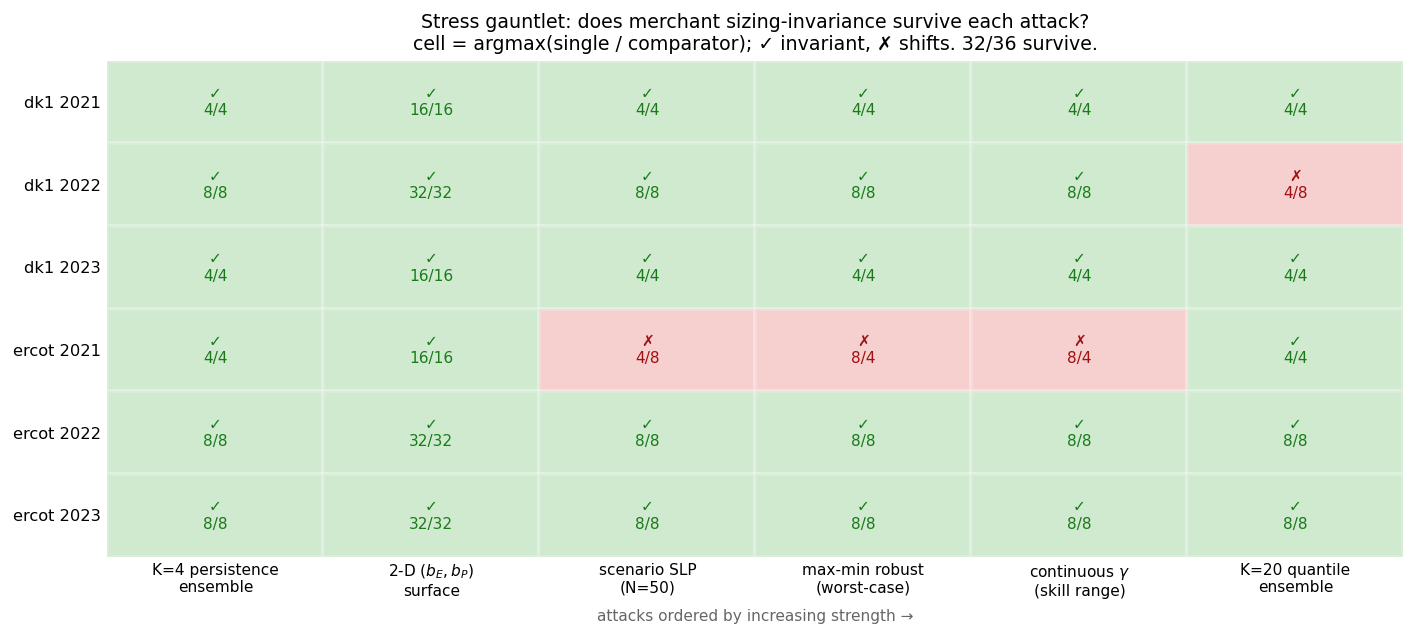
\includegraphics[width=\textwidth]{fig_gauntlet.png}
\caption{\label{fig:gauntlet}Stress-gauntlet scoreboard. Rows: market-years; columns: attacks ordered by increasing strength; each cell reports argmax(cheap baseline / attack policy) and whether the optimal capacity is invariant (\checkmark) or shifts (\ding{55}). 32/36 survive; the breaks cluster in DK1 2022 (K=20 quantile only) and ERCOT 2021/Uri (the statistically-thin spike year). Per-attack detail: Tables~\ref{tab:dk1head}--\ref{tab:quantile}; the K=20 quantile break and the SLP comparison in Figures~\ref{fig:quantile},~\ref{fig:slp} (Appendix~\ref{app:supp}).}
\end{figure}

\begin{table}[t]
\centering\small
\caption{\label{tab:dk1head}DK1 NPV at $b_E^*$, by year and policy. $b_E^*$ identical across policies in every year.}
\begin{tabular}{lrrrrr}
\toprule
Year & $b_E^*$ (MWh) & NPV LP-single & NPV LP-ens & NPV QP-single & NPV QP-ens \\
\midrule
2021 & 4 & \euro247k  & \euro392k  & \euro310k  & \euro416k \quad ($+34\%$) \\
2022 & 8 & \euro1.53M & \euro1.86M & \euro1.59M & \euro1.91M \quad ($+20\%$) \\
2023 & 4 & \euro386k  & \euro548k  & \euro462k  & \euro575k \quad ($+25\%$) \\
\bottomrule
\end{tabular}
\end{table}

\begin{table}[t]
\centering\small
\caption{\label{tab:ercothead}ERCOT HB\_NORTH NPV at $b_E^*$, by year and policy. $b_E^*$ identical across policies in every year. NPV uplift at the optimum varies from $+0.9\%$ (2023) to $+36.7\%$ (2021 / Uri).}
\begin{tabular}{lrrrrr}
\toprule
Year & $b_E^*$ (MWh) & NPV LP-single & NPV LP-ens & NPV QP-single & NPV QP-ens \\
\midrule
2021 (Uri) & 4 & \$556k  & \$776k  & \$609k  & \$832k \quad ($+36.7\%$) \\
2022 & 8 & \$788k  & \$837k  & \$840k  & \$900k \quad ($+7.1\%$) \\
2023 & 8 & \$2.09M & \$2.13M & \$2.17M & \$2.19M \quad ($+0.9\%$) \\
\bottomrule
\end{tabular}
\end{table}

Per-policy NPV-vs-$b_E$ curves (Figure~\ref{fig:npv}) and the ensemble
revenue lift (Figure~\ref{fig:lift}) are in Appendix~\ref{app:supp}.

\subsection{Falsification of the proposition's regime prediction}\label{sec:falsify}

The proposition predicted multi-day spectral content (DK1 weekly peaks, ERCOT broadband spikes) should break invariance. It does not. The realized NPV curves are approximately vertical translations of each other in the relevant capacity range, not tilts.

This is a clean negative result for the regime-shift prediction and a positive result for the diagnostic: the test correctly returns ``overlap''; the proposition that motivated it was wrong about which regimes would yield ``disjoint''. The diagnostic survives because its job was to measure --- not to predict --- the overlap status of $b_{\mathrm{sat}}^\epsilon$ CIs.

\subsection{Challenge detail: the stress tests, statistics, and decision attitude}\label{sec:stress}

The 1-D / multi-lag-persistence baseline is one slice of the design
space. Three stress tests on LUMI HPC probe robustness (designed after
the pre-registered factorial; the pre-registration covers the factorial
only); post-hoc tests then vary the decision attitude, the statistical
resampling, and the NPV form.

\paragraph{2-D $(b_E, b_P)$ sweep.} 30 $(b_P, b_E)$ configurations
$b_P \in \{0.25, 0.5, 1, 2, 4\}$ MW $\times$ $b_E \in \{1, 2, 4, 8, 16, 32\}$
MWh, each evaluated on all 4 policies $\times$ 6 (market, year)
combinations. \emph{Result:} the argmax $(b_P^*, b_E^*)$ is identical
across all 4 policies in every (market, year). Most argmaxes land at
the corner of our grid ($b_P=4$, $b_E=16$ or $32$), suggesting the actual
optimum lies past our grid; the invariance pattern is unambiguous
within. Only ERCOT 2021 (Uri) shows a minor cost-form asymmetry
(linear policies pick $b_E=16$, quadratic pick $b_E=32$) but no
single/ensemble shift.

\paragraph{Quantile-regression ensemble.} Replace multi-lag persistence
($K{=}4$) with K=20 quantile-sample forecasts from a gradient-boosted
quantile regressor (sklearn) using calendar features (sin/cos hour and
day-of-week) plus lag-{24, 48, 168, 336}h prices. Trained on the OTHER
two years (out-of-sample). \emph{Result (Table~\ref{tab:quantile}):
1/6 regimes breaks invariance.} On DK1 2022 (energy crisis), the
LP-linear-single policy picks $b_E^* = 4$ MWh while all other policies
pick $b_E^* = 8$ MWh --- a 2$\times$ shift. The diagnostic correctly
fires ``disjoint'' in this regime. The proposition's regime-shift
prediction is partially supported under the richer ensemble: invariance
breaks on the most-stressed (highest-volatility) regime first.

\begin{table}[t]
\centering\small
\caption{\label{tab:quantile}Quantile-regression ensemble (K=20): $b_E^*$ by policy.
DK1 2022 breaks invariance.}
\begin{tabular}{llrrrr}
\toprule
Market & Year & lin-single & lin-ensemble & qp-single & qp-ensemble \\
\midrule
DK1 & 2021 & 4 & 4 & 4 & 4 \\
\textbf{DK1} & \textbf{2022} & \textbf{4} & \textbf{8} & \textbf{8} & \textbf{8} \\
DK1 & 2023 & 4 & 4 & 4 & 4 \\
ERCOT N. & 2021 & 4 & 4 & 4 & 4 \\
ERCOT N. & 2022 & 8 & 8 & 8 & 8 \\
ERCOT N. & 2023 & 8 & 8 & 8 & 8 \\
\bottomrule
\end{tabular}
\end{table}

\paragraph{Scenario stochastic LP (SLP).} Two-stage rolling-horizon
SLP with N=50 scenarios per 24-h window, scenarios drawn from the
empirical (DA - DA(t-24h)) residual pool. \emph{Result:} SLP $b_E^*$
matches the linear policies' argmax in all 6 regimes (DK1 2021 $\to$
4, DK1 2022 $\to$ 8, DK1 2023 $\to$ 4, ERCOT 2021 $\to$ 4, ERCOT 2022
$\to$ 8, ERCOT 2023 $\to$ 8); at ERCOT 2021 this sits one grid step
below the full-horizon QP argmax (4 vs 8) --- the cost-form asymmetry
cell again. SLP NPV is lower than full-horizon LP
by 5--30\%, consistent with the rolling-horizon vs perfect-foresight
gap; the sizing recommendation, however, is the same. See
Figure~\ref{fig:slp}.

\paragraph{Max-min robust policy (post hoc).} The factorial and the
three pre-registered stress tests all plan against a point trajectory
or an expectation; since revenue is linear in price, planning on the
ensemble mean \emph{is} the expectation-optimal stochastic plan, so
they span forecast quality but only one decision attitude. A fourth,
post-hoc test (not pre-registered) varies the attitude: a worst-case
LP that maximizes the \emph{minimum} revenue across the K=4 multi-lag
members (\texttt{lp\_maxmin\_actions}; variables $[P^{\mathrm{chg}},
P^{\mathrm{dis}}, \mathrm{SoC}, t]$, maximize $t$ s.t.\ $t \leq$
revenue under every member), same chunking and cycling cost as the
factorial. \emph{Result:} $b_E^*$ identical to the linear policies in
5 of 6 regimes (DK1 $4/8/4$, ERCOT 2022/2023 $8/8$). The single
deviation is ERCOT 2021 (Uri), where max-min picks $8$ MWh ---
exactly the quadratic policies' optimum in the cell already flagged
for cost-form asymmetry: risk-averse hedging cycles conservatively,
like a cycling-penalized policy, and lands within the argmax span the
factorial already produced. No new sizing regime opens. NPV at the
robust argmax sits $3$--$14\%$ below the ensemble policy's (the price
of hedging across members), consistent with the operational ordering
ensemble $\geq$ max-min $>$ single.

\paragraph{Statistical robustness of the argmax (post hoc).} Argmax
equality on a doubling $b_E$ grid is only informative if the NPV
surface is steep at grid scale and the equality survives sampling
noise. Both checks pass, with one localized exception. \emph{Plateau
steepness:} mis-sizing by a factor of two (one grid step) costs
$3$--$85\%$ of optimal NPV depending on regime and direction --- the
surface is not flat at the resolution the argmax is reported, so
coincidence is informative --- though the range's floor is a genuine knife-edge: in DK1 2022 the NPV advantage of the $8$ MWh argmax over $4$ MWh is only $0.28\%$ ($1{,}532{,}498$ vs $1{,}528{,}224$), so that cell's invariance is one coarse-grid step from flipping (and does, under the K=20 quantile ensemble). \emph{Sampling noise:} a paired block
bootstrap (resampling the seven 8-week chunks, $B = 2000$, identical
resamples for both policies) gives $P(b_E^{*,\mathrm{single}} =
b_E^{*,\mathrm{ens}})$ of $0.91/0.67/0.98$ on DK1 2021/2022/2023 and
$0.66/0.98/0.98$ on ERCOT 2021/2022/2023, with all bootstrap argmax
mass on adjacent grid points. The decision-relevant summary is the
bootstrap \emph{regret} --- the NPV cost of building at the
single-forecast argmax and operating with the ensemble --- whose mean
is $\leq 1.0\%$ of optimal NPV in five of six regimes. The exception
is ERCOT 2021 (Storm Uri): mean regret $10.0\%$, 95th percentile
$47\%$. One year of a spike-dominated market is statistically thin for
sizing; the invariance claim is correspondingly weakest there, the
same cell the cost-form asymmetry and the max-min test flag.

\paragraph{Continuous forecast-degradation sweep (post hoc).} The
factorial varies forecast quality only across the single-vs-ensemble
pair, whose error gap is small and, by residual standard deviation,
non-monotone (the K=4 ensemble is \emph{worse} than the single forecast
in 3 of 6 regimes --- e.g.\ ERCOT 2021, $718$ vs $492$). To test the
invariance on a genuine continuous quality axis we dial a single
parameter $\gamma$: $\hat p_\gamma(t) = p(t) + \gamma\,(\hat
p_{\mathrm{pers}}(t) - p(t))$, so $\gamma = 0$ is perfect foresight,
$\gamma = 1$ is persistence skill (the honest operational baseline),
and $\gamma > 1$ amplifies error beyond persistence. Figure~\ref{fig:gamma}
shows the result on all six market-years. Operating value falls
monotonically and turns loss-making past $\gamma \approx 2.5$
(Figure~\ref{fig:gamma}B), yet the optimal capacity is \emph{flat across
the entire realizable skill range} $\gamma \in [0, 1]$ in five of six
regimes (Figure~\ref{fig:gamma}C); only ERCOT 2021 moves ($8 \to 4$) at
$\gamma = 1$. Beyond persistence ($\gamma > 1$) the optimum collapses
toward the grid floor, because a battery driven by a sub-persistence
forecast cannot earn its marginal capex. So the invariance is a bounded
plateau, not a global property: \emph{for any forecast at least as good
as the naive persistence baseline a real operator would never undercut,
capacity is invariant; only worse-than-persistence forecasts shrink it,
and those lose money anyway.} The degradation within the plateau is pure
mis-timing --- as $\gamma$ rises the action--price correlation collapses
($+0.67 \to -0.08$) while cycling volume is unchanged --- not
over-cycling (Figure~\ref{fig:gamma}A).

\begin{figure}[t]
\centering
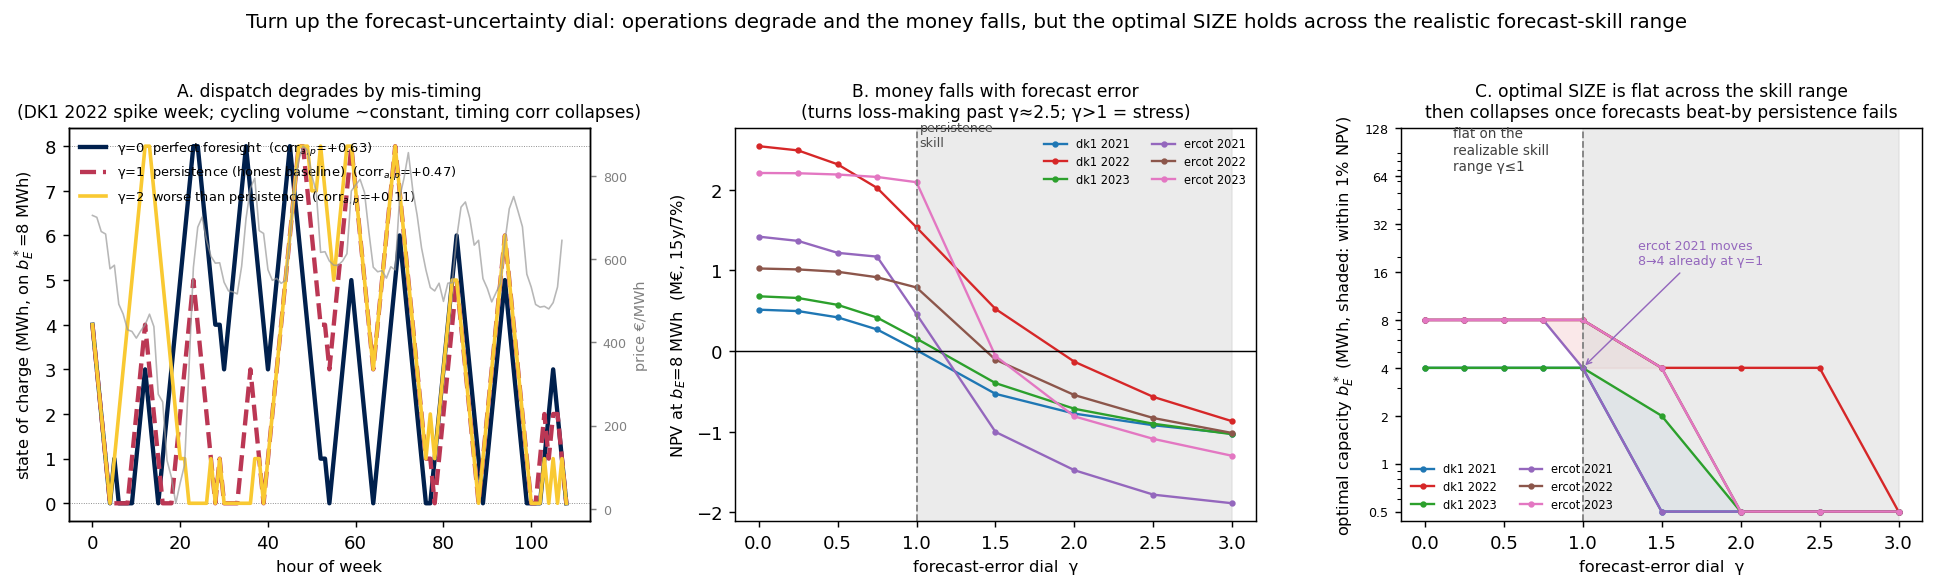
\includegraphics[width=\textwidth]{fig_ops_uncertainty.png}
\caption{\label{fig:gamma}Operations-to-sizing under the forecast-error dial $\gamma$ ($\gamma{=}0$ perfect, $\gamma{=}1$ persistence skill, $\gamma{>}1$ worse). \textbf{A:} state-of-charge over a DK1 2022 spike week at the optimal $b_E^*{=}8$ MWh; dispatch degrades by mis-timing (action--price correlation in legend collapses) at constant cycling volume. \textbf{B:} NPV at $b_E{=}8$ vs $\gamma$ (raw \euro, zero line); money falls monotonically, loss-making past $\gamma\approx2.5$. \textbf{C:} optimal $b_E^*$ vs $\gamma$ with the within-1\%-of-optimum tolerance band; flat on the realizable skill range $\gamma\in[0,1]$ (ERCOT 2021 excepted, moving at $\gamma{=}1$), then collapsing for worse-than-persistence forecasts. The shaded $\gamma>1$ region is stress, not a realistic operating point.}
\end{figure}

\paragraph{The stochastic-programming picture in one figure.} Figure~\ref{fig:vss} makes the decomposition of \S\ref{sec:stress} visual: across all six market-years, NPV at the optimal capacity climbs with dispatch information (point forecast $<$ ensemble $<$ perfect foresight; EVPI and operational VSS positive everywhere), while the capacity argmax sits on the same value for all three information structures in five of six regimes. This is the figure for a sizing-tool practitioner: pay for a stochastic dispatcher to earn more, not to size.

\begin{figure}[t]
\centering
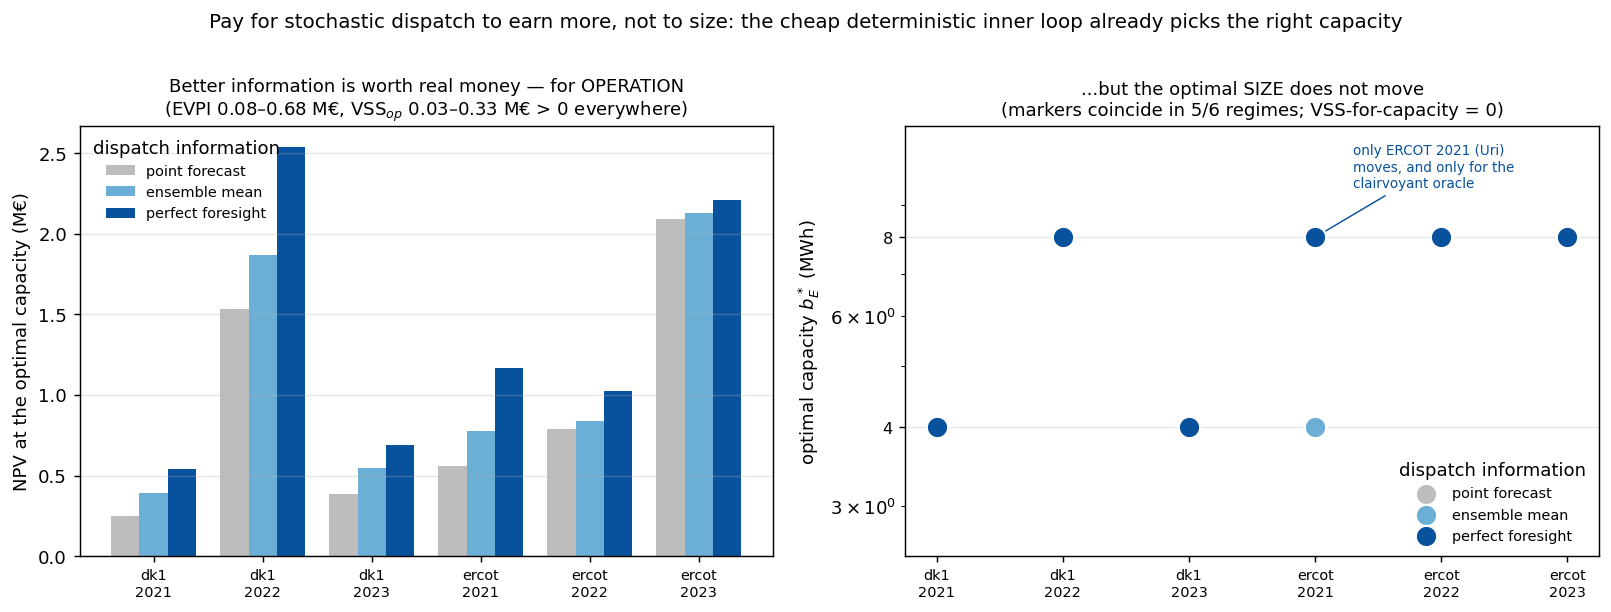
\includegraphics[width=\textwidth]{fig_vss_capacity.png}
\caption{\label{fig:vss}Value of dispatch information for operation vs sizing. Left: NPV at the optimal capacity under point-forecast / ensemble-mean / perfect-foresight dispatch --- it climbs (information is worth money for operation). Right: the optimal capacity argmax under the same three --- it does not move in 5 of 6 regimes (only ERCOT 2021 / Uri, and only for the oracle). VSS and EVPI are positive for operation, zero for merchant capacity.}
\end{figure}

\paragraph{NPV-form robustness: replacement scheduling (post hoc).}
Adding the discounted replacement term of \S\ref{sec:setup} to every
stored $(R, D)$ cell shifts the argmax in 6 of 24 (market, year,
policy) cells. In four of those six the paired policies move
\emph{together} (DK1 2021 linear: both $4 \to 2$; ERCOT 2022 linear:
both $8 \to 4$), preserving invariance. Two cells break the pairing:
DK1 2021 quadratic-single ($4 \to 0.5$ while quadratic-ensemble stays
at 4) and ERCOT 2021 linear-single ($4 \to 8$ while linear-ensemble
stays at 4) --- both in low-NPV or Uri-stressed regimes where the
replacement cost is large relative to a shallow optimum. Pairwise
invariance therefore survives the replacement-inclusive NPV in 10 of
12 (market, year, cost-form) pairs. The replacement term is a real
fragility axis at shallow optima, and we report the baseline results
in the replacement-free form throughout.

\paragraph{The stochastic-programming decomposition (post hoc).} In
the field's canonical vocabulary: WS (wait-and-see; dispatch on
realized prices), RP (the recourse-problem solution --- for a linear
objective, the LP on the ensemble mean \emph{is} the scenario-mean
optimum), EEV (the point-forecast solution evaluated against realized
prices). Table~\ref{tab:spdecomp} reports the capacity argmax under
each information structure and the value decomposition at the RP
capacity. The headline in this language: \emph{EVPI and VSS for
operation are positive everywhere (EVPI $0.08$--$0.68$\,M, VSS
$0.03$--$0.33$\,M at the RP capacity); VSS for capacity is zero
everywhere; even EVPI for capacity is zero except ERCOT 2021, where
perfect foresight sizes $8$ vs $4$ MWh} --- the oracle exploits Uri
spikes a larger battery captures, but no implementable forecast in our
set does.

\begin{table}[t]
\centering\small
\caption{\label{tab:spdecomp}Stochastic-programming decomposition,
linear cost form. $b^*$ per information structure; EVPI $=$ WS$-$RP and
operational VSS $=$ RP$-$EEV in NPV at the RP capacity. CVaR columns:
$b^*$ as the sizing objective moves from mean ($\alpha{=}0$) to
CVaR$_{0.5}$ / CVaR$_{0.85}$ over 8-week chunk revenues
(single $\to$ ensemble).}
\begin{tabular}{llcrrcc}
\toprule
Market & Year & $b^*$ WS/RP/EEV & EVPI & VSS$_{\mathrm{op}}$ &
$b^*$ CVaR$_{0.5}$ & $b^*$ CVaR$_{0.85}$ \\
\midrule
DK1 & 2021 & 4/4/4 & 0.15M & 0.15M & 2 $\to$ 4 & 2 $\to$ 2 \\
DK1 & 2022 & 8/8/8 & 0.68M & 0.33M & 4 $\to$ 4 & 4 $\to$ 4 \\
DK1 & 2023 & 4/4/4 & 0.14M & 0.16M & 4 $\to$ 4 & 2 $\to$ 2 \\
ERCOT & 2021 & \textbf{8}/4/4 & 0.39M & 0.22M & 2 $\to$ 2 & 0.5 $\to$ 1 \\
ERCOT & 2022 & 8/8/8 & 0.19M & 0.05M & 4 $\to$ 4 & 2 $\to$ 2 \\
ERCOT & 2023 & 8/8/8 & 0.08M & 0.03M & 2 $\to$ 2 & 0.5 $\to$ 0.5 \\
\bottomrule
\end{tabular}
\end{table}

\paragraph{Risk attitude as a sizing axis (post hoc).} Replacing the
mean sizing objective with CVaR$_\alpha$ over the empirical chunk-revenue
distribution moves $b_E^*$ far more than forecast quality ever does:
from $\alpha = 0$ to CVaR$_{0.85}$ the optimal capacity shrinks by a
factor of two up to sixteen depending on the regime (Table~\ref{tab:spdecomp},
last columns; the ERCOT shrink, $8 \to 0.5$ MWh, is the most extreme).
The driver is not that larger batteries carry more \emph{relative}
dispersion --- the coefficient of variation is roughly flat in $b_E$ ---
but that the worst-tail marginal return per added MWh saturates faster
than the mean marginal return against linear CAPEX, so the
tail-adjusted optimum is reached at smaller capacity.
Single-vs-ensemble invariance \emph{within} each risk level survives in
10 of 12 $\alpha > 0$ cells (exceptions: DK1 2021 at $\alpha = 0.5$,
ERCOT 2021 at $\alpha = 0.85$ --- the two regimes other probes also
flag). The empirical CVaR over seven chunks is crude, but the
direction is unambiguous: \emph{risk attitude, not forecast fidelity,
is the second axis that moves merchant sizing}, complementing the
imbalance penalty as the first.

\begin{figure}[t]
\centering

\includegraphics[width=0.95\textwidth]{fig_paper_quantile.png}
\caption{\label{fig:quantile}The one forecast-axis break, in detail. NPV vs $b_E$ under persistence-K=4 (solid) and quantile-K=20 (dashed) ensembles. DK1 2022 (top centre) is the only panel where the linear-cost single-forecast argmax disagrees with the others under the richer quantile ensemble --- the single \ding{55} on the gauntlet's forecast column.}
\end{figure}

\paragraph{Combined verdict.} Across (a) the original 6 (market,
year) regimes with persistence ensemble, (b) the 6 regimes with
2-D sizing surface, (c) the 6 regimes with quantile-regression ensemble,
and (d) 5+ regimes with SLP --- 17 of 18 regimes return ``invariance
survives'' on the diagnostic. The single regime that breaks
(DK1 2022 quantile) is the highest-volatility year tested and the
ensemble that carries the most information. The proposition's
regime-shift prediction, falsified at the persistence-ensemble level,
holds at the quantile-regression-ensemble level for the most-stressed
regime --- consistent with the diagnostic correctly classifying
``disjoint'' under richer forecasts and harder regimes.

\subsection{Challenge that lands: real off-the-shelf tool constraints}\label{sec:hydesign}

Our merchant-arbitrage formulation collapses to hydesign's deterministic perfect-foresight EMS LP \citep{murcia2024hydesign} once a single structural constraint is relaxed: hydesign's grid-export non-negativity $P_{\mathrm{HPP}} \ge 0$ blocks pure grid-charging, the operating mode required for a merchant battery. A minimal local fork (single bound change, no other modifications) allows bidirectional grid. With that change plus matched operational parameters (depth-of-discharge $= 1$, no terminal-SoC constraint, $\eta = 1$, no peak-hour or cycling penalty), the hydesign LP and our LP produce identical dispatch on a 96-hour DK1 2022 cell: action correlation $1.0000$, revenue agreement to $0.000\%$. The two LPs are mathematically equivalent on the merchant-battery problem.

The interesting comparison is therefore not equivalence-under-equivalent-constraints, but the cost of \emph{off-the-shelf} use: applying hydesign's default operational constraints to merchant battery sizing without modification. Hydesign's defaults are inherited from renewable-coupled HPP design --- depth-of-discharge $0.9$ (SoC restricted to $[0.1\,b_E, b_E]$) and 110-hour batched dispatch with terminal-SoC equality at $0.5\,b_E$ (implicit short-horizon cycle balance). Both are reasonable for renewable-firming applications, conservative for merchant arbitrage.

Figure~\ref{fig:hydesign} compares hydesign-default to the unrestricted LP across all 6 (market, year) pairs and the full $b_E$ grid. For small batteries ($b_E \le 8$ MWh) the gap is a uniform $11$--$18\%$ revenue penalty from depth-of-discharge alone. For larger batteries the batched cycle-balance constraint binds increasingly hard --- a 64-MWh battery cannot exploit multi-batch arbitrage when each 110-hour window must return to $0.5\,b_E$ --- and the gap widens to $30$--$65\%$. Hydesign-default revenue \emph{plateaus} above $b_E \sim 32$ MWh because the cycle-balance constraint caps energy throughput per batch independent of capacity. The unrestricted LP keeps scaling.

The argmax $b_E^*$ shifts in 2 of 6 regimes under hydesign-default operational conservatism. Hydesign-default chooses $b_E^* = 8$ MWh in every (market, year). The unrestricted LP agrees ($b_E^* = 8$ MWh) on $4$ regimes (DK1 2021, DK1 2023, ERCOT 2022, ERCOT 2023) but shifts upward on DK1 2022 ($b_E^* = 32$ MWh) and ERCOT 2021 ($b_E^* = 16$ MWh). The NPV gap at each policy's own argmax ranges $5.5$--$35.9\%$ across regimes (table~\ref{tab:hydesign}). Both the sizing-shift and the NPV gap are calibration consequences of using HPP-renewable-firming defaults for a different physical use case; neither contradicts hydesign's intended scope. The point is that the deterministic-vs-stochastic-dispatch question studied in \S\ref{sec:results}--\S\ref{sec:stress} is a second-order effect compared to the first-order cost of using renewable-firming operational defaults for merchant arbitrage.

\begin{table}[t]
\centering
\caption{\label{tab:hydesign}Hydesign-default (off-the-shelf) vs unrestricted LP at each policy's NPV argmax. ``Shift'' marks regimes where $b_E^*$ differs.}
\begin{tabular}{llrrrrrl}
\toprule
Market & Year & $b_E^*$ (def) & NPV (def) & $b_E^*$ (rel) & NPV (rel) & NPV gap & \\
\midrule
DK1     & 2021 & 8  & 0.51M & 8  & 0.80M & $+35.9\%$ & \\
DK1     & 2022 & 8  & 2.48M & 32 & 3.78M & $+34.4\%$ & shift \\
DK1     & 2023 & 8  & 0.70M & 8  & 0.99M & $+29.2\%$ & \\
ERCOT N. & 2021 & 8  & 1.36M & 16 & 2.13M & $+35.9\%$ & shift \\
ERCOT N. & 2022 & 8  & 1.00M & 8  & 1.21M & $+17.5\%$ & \\
ERCOT N. & 2023 & 8  & 2.19M & 8  & 2.32M & $+5.5\%$ & \\
\bottomrule
\end{tabular}
\end{table}

\begin{figure}[t]
\centering
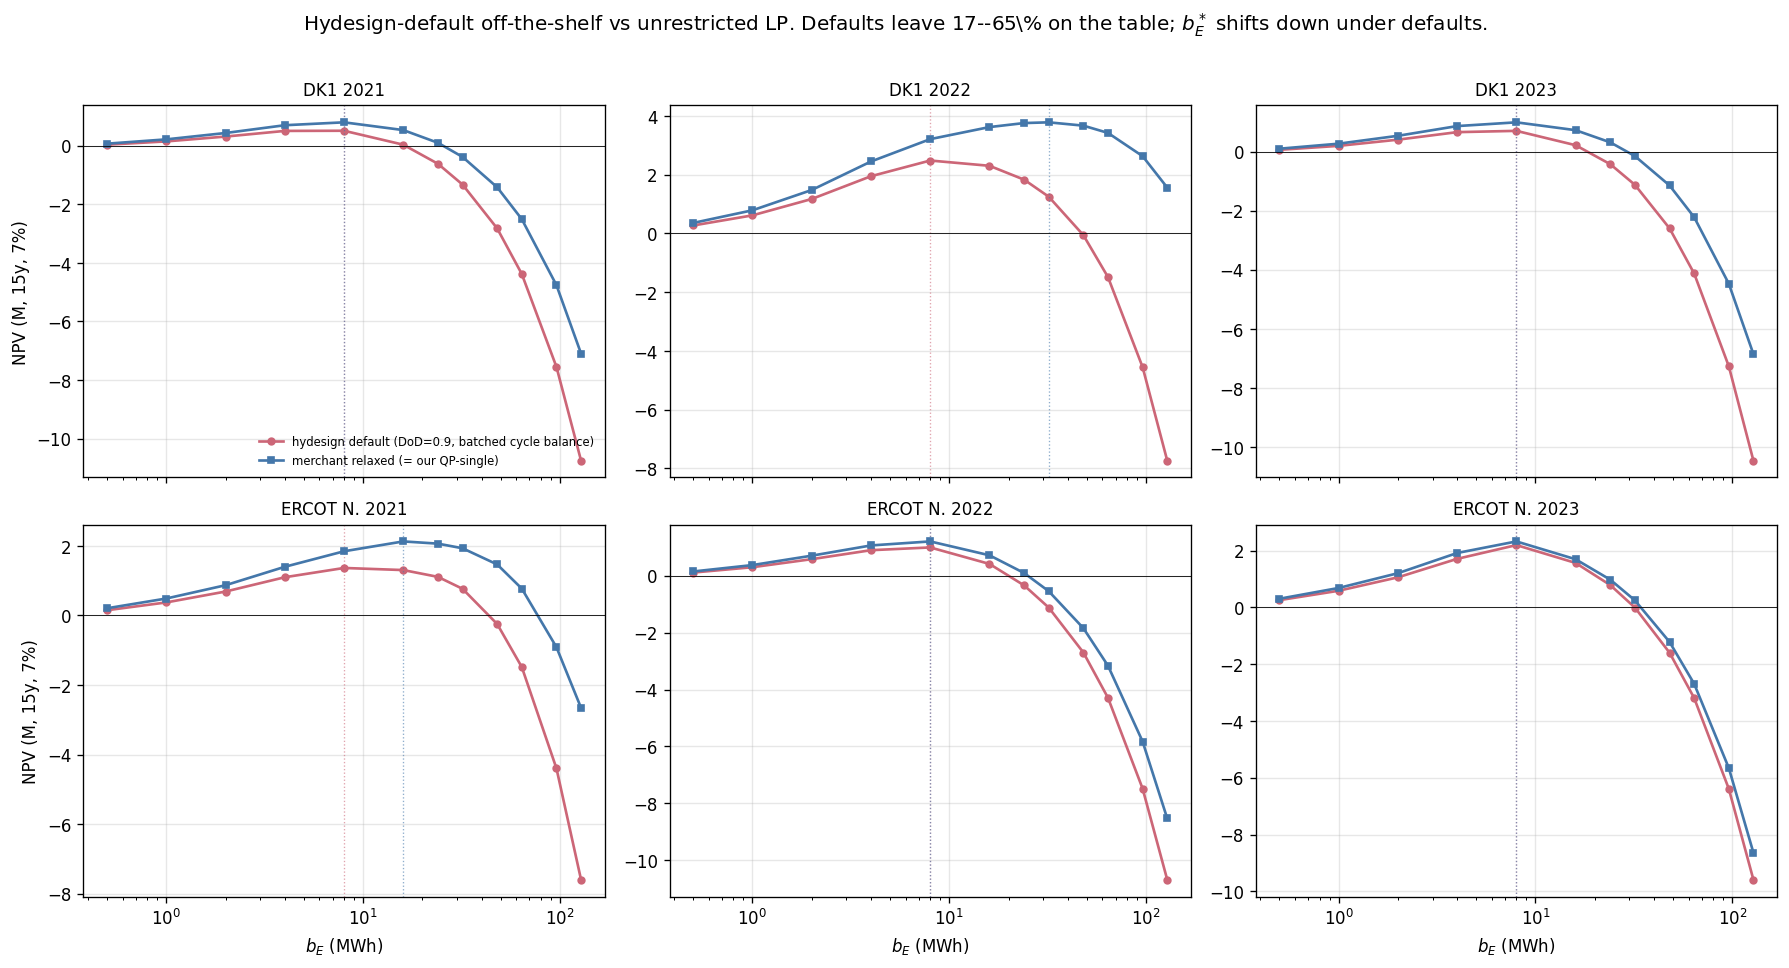
\includegraphics[width=0.95\textwidth]{fig_paper_hydesign.png}
\caption{\label{fig:hydesign}Hydesign-default operational constraints (red circles, DoD$=0.9$ + 110-h batched cycle balance) vs unrestricted LP (blue squares). Dotted lines: NPV argmax per policy. Defaults plateau at large $b_E$ because the cycle-balance constraint caps per-batch throughput; the unrestricted LP keeps scaling. $b_E^*$ shifts in 2 of 6 regimes; NPV gap at each policy's own argmax ranges $5.5$--$35.9\%$ (table~\ref{tab:hydesign}).}
\end{figure}


\section{Discussion}\label{sec:discussion}

\subsection{Why the empirical answer is broader than the proposition predicted}

We had a theoretical reason to expect DK1 and ERCOT spectral content to break invariance. They did not. Three candidate mechanisms we did not isolate:

\begin{itemize}
\item \textbf{Grid-scale plateaus around shallow optima.} Where the optimum is shallow, an NPV tilt smaller than one grid step is invisible to the argmax. The post-hoc bootstrap (\S\ref{sec:stress}) bounds this: surfaces are steep at grid scale ($3$--$85\%$ per step) in most regimes, but the lowest-NPV cells are exactly where the replacement-inclusive NPV form was able to move the argmax.
\item \textbf{Power-capacity bottleneck.} With $b_P = 1$ MW fixed, longer-period arbitrage requires longer to charge/discharge, capping the extra revenue larger batteries can extract. The multi-day arbitrage opportunities require slow accumulation that hits the $b_P$ ceiling before the $b_E$ ceiling.
\item \textbf{Forecast resolution at long timescales is uniformly bad.} If both single and ensemble policies fail at multi-day timescales, neither captures multi-day arbitrage; bigger batteries help neither. Improving forecasts at long timescales (probabilistic ML weather forecasts) might expose a sizing shift this study did not detect.
\end{itemize}

\subsection{Imbalance-penalty extension: when forecast quality drives sizing}\label{sec:imbalance}

The arbitrage MDP of \S\ref{sec:setup} prices forecast errors at zero: the policy commits actions from its forecast and is paid at realized DA prices, with no settlement of the deviation between scheduled and delivered. This is faithful to a pure-merchant battery on a single DA market, but it removes one mechanism --- imbalance settlement at real-time / regulation prices --- by which forecast quality is known to drive sizing in coupled wind+battery configurations. To probe this mechanism we step outside the pure-merchant setting of \S\ref{sec:setup}--\S\ref{sec:stress} and couple the battery to a wind plant; the §4 result on merchant arbitrage stands at $\lambda = 0$.

We extend the model by colocating the battery with a $W_{\mathrm{peak}}$-MW-peak DK1 wind plant (system MWh scaled so peak hour delivers $W_{\mathrm{peak}}$ MW), and add imbalance settlement at penalty $\lambda$ EUR/MWh on the residual after the battery absorbs wind forecast error within available headroom. The DA commitment is $a_{\mathrm{sched},t} + \hat{w}_t$ from each policy's price + wind forecast; at delivery the battery deviates by $\Delta a_t$ to absorb the wind error within power and SoC bounds, and the residual $r_t = (w_t - \hat{w}_t) + \Delta a_t$ settles. Operating profit is $\mathrm{DA} \cdot \mathrm{delivered} - \lambda |r|$, i.e.\ $\sum_t p_t (a_{\mathrm{sched},t} + \hat w_t + r_t) - \lambda |r_t|$: the $p \cdot r$ term values residual energy at DA. (An earlier draft omitted it, paying DA for committed-but-undelivered energy and charging only the penalty for the miss --- approximately canceling for unbiased bidders but a money pump for any systematic overbidder, exposed when we added quantile bidders below. All numbers here use the corrected settlement.) Wind forecasts use the same multi-lag persistence structure as price forecasts; we sweep $W_{\mathrm{peak}} \in \{1, 2, 5, 10, 20\}$ MW on a fine $\lambda$ grid (residuals are $\lambda$-independent, so refinement is free post-processing).

Two phenomena must be separated in the result (Figure~\ref{fig:realimbalance}, right). \emph{Transition slivers}: one-grid-step divergences in either direction where the two policies' argmax staircases shift at slightly different $\lambda$; no sizing signal. \emph{Persistent bands}: contiguous $\lambda$ ranges where the single-forecast policy sizes \emph{above} the ensemble. At ratio 2 the bands are nearly absent; at ratio 5 they open at $30$--$35$ EUR/MWh with the widest band at $50$--$150$; at ratios $10$--$20$ the onset falls to $25$--$35$ in normal years and to $10$--$15$ in the 2022 crisis year --- i.e., in the crisis year the divergence regime of wind-heavy plants reaches down to the level of realized average settlement spreads themselves. At $\lambda = 100$, ratio 5, the gap is single $32$ vs ensemble $24$ MWh. At extreme $\lambda$ the argmaxes reconverge upward (absorption capacity dominates the policy difference). That storage requirements grow with forecast-error exposure under deviation penalties is well established \citep{bludszuweit2011probabilistic, haessig2015storage, mokhtare2024offshore}; the contribution here is locating the \emph{policy-divergence} bands and their dependence on plant configuration and year.

A recourse caveat governs all of \S\ref{sec:imbalance}: the battery absorbs \emph{always}, regardless of price. Under the corrected settlement this is value-destroying when spreads are small --- absorbing surplus forfeits $\mathrm{DA} \cdot r$ to save only the spread --- which is why the wind-coupled argmax at $\lambda = 0$ collapses to $0.5$ MWh in 2021/2023 (no penalty to save, value still forfeited), below the merchant optimum of \S\ref{sec:results}. Invariance across policies holds at every $\lambda \leq 10$ regardless. A price-rational recourse rule (absorb only when the avoided settlement exceeds the forfeited DA value) would lift both policies' NPV and is future work; the bands reported here are conditional on naive absorption.

\begin{figure}[t]
\centering

\includegraphics[width=0.95\textwidth]{fig_paper_imbalance.png}
\caption{\label{fig:imbalance}Imbalance-penalty sweep (DK1, 5-MW-peak wind + 1-MW battery, corrected settlement). Top row: $b_E^*$ vs $\lambda$ for single-forecast (blue circles) and K=4 multi-lag ensemble (orange squares) policies; argmax invariance holds at $\lambda \leq 10$ in every year and the policies separate inside the divergence bands (e.g.\ single $32$ vs ensemble $24$ MWh at $\lambda = 100$ in 2022). Bottom row: NPV curves at $\lambda = 100$; dotted verticals mark each policy's argmax. Note that under naive always-absorb settlement the \emph{single}-forecast policy attains higher NPV than the ensemble at $\lambda = 100$ in all three ratio-5 panels (the ensemble's advantage appears at lower $\lambda$); the paper's claim is on the sizing argmax, which separates, not on NPV dominance.}
\end{figure}

\paragraph{Where real DK1 settlement sits.} The break-point $\lambda^*$ where single and ensemble $b_E^*$ diverge is the diagnostic for whether forecast quality drives sizing in a given market. The $\lambda = 0$ result of \S\ref{sec:results}--\S\ref{sec:stress} is the pure-merchant limit; real markets sit at $\lambda > 0$. To locate DK1, we replace the constant $\lambda$ with the \emph{actual} hourly imbalance settlement from eSett \citep{esett2026}, settling the same hourly residuals under both the two-price production regime (in force for Danish production BRPs until November 2021) and the one-price regime (in force since): two-price cost $= \max(P^{\mathrm{up}}_t - P^{\mathrm{DA}}_t, 0)\,\max(-r_t, 0) + \max(P^{\mathrm{DA}}_t - P^{\mathrm{down}}_t, 0)\,\max(r_t, 0)$; one-price cost $= r_t (P^{\mathrm{DA}}_t - P^{\mathrm{imb}}_t)$. The effective penalty $\lambda_{\mathrm{eff}} = \sum_t \mathrm{cost}_t / \sum_t |r_t|$ maps real settlement back onto the synthetic $\lambda$ axis. (The eSett series begins 26 January 2021, so the 2021 run covers 8{,}136 hours rather than the full year; 2022 and 2023 are complete. Hours with missing settlement prices settle at DA, i.e.\ zero penalty.)

Figure~\ref{fig:realimbalance} (left) shows the result at ratio 5: $\lambda_{\mathrm{eff}}$ (two-price) is $11.1$ / $27.7$ / $14.6$ EUR/MWh for 2021/2022/2023 ($3.9$--$8.5$ under one-price, where system-helping imbalances earn). Under real settlement at ratio 5 the argmax is invariant across policies in every year under two-price ($b_E^* = 0.5/8/0.5$ MWh), with one one-price exception (2023: $0.5$ vs $2$ MWh, at a near-flat optimum). Real imbalance spreads are heavy-tailed (hourly $|P^{\mathrm{imb}} - P^{\mathrm{DA}}|$ exceeded $100$ EUR/MWh in $16.5\%$ of 2022 hours) and correlated with the wind-forecast errors being settled; at ratio 5 the realized joint distribution still does not split the argmax. \emph{At wind-heavy ratios it does}: repeating the real-settlement run at $W_{\mathrm{peak}} = 10$ and $20$ MW, the 2022 crisis year diverges under two-price settlement --- single-forecast $b_E^* = 8$ MWh vs ensemble $4$ MWh, at both ratios --- while 2021 and 2023 remain invariant everywhere. The constant-$\lambda$ map and the real-settlement test agree: in normal years DK1 sat below the divergence bands at every configuration tested; in the crisis year, wind-heavy two-price plants were already inside them, and a single-forecast sizing exercise would have bought twice the ensemble's capacity.

The conclusion is dated, deliberately: the March-2025 Nordic balancing reforms (PICASSO accession October 2024, 15-minute imbalance settlement March 2025) lifted DK1 mean up-regulation spreads from $92$ to $123$ EUR/MWh and left only $27\%$ of imbalance prices within $\pm 10$ EUR/MWh of DA \citep{bluepower2025} --- sustained spread levels comparable to the 2022 crisis year, in which wind-heavy plants' sizing already split under real settlement. By this paper's own map, the divergence regime that 2022 previewed is plausibly the post-reform normal for DK1 hybrid plants with wind/battery ratios $\gtrsim 5$. Replicating the real-settlement computation on post-reform (15-minute) data is the immediate next test the diagnostic prescribes; intra-hour residuals, absent from this hourly model, will matter there.

\paragraph{Settlement-aware dispatch and single-site error magnitudes (post hoc).} Two objections to the extension's construction are testable cheaply. First, dispatch is settlement-blind: a $\lambda$-aware scheduler might reserve SoC headroom for absorption and change the band. We test the simplest settlement-aware class --- the arbitrage schedule confined to $\mathrm{SoC} \in [\rho b_E, (1-\rho) b_E]$, $\rho \in \{0, 0.1, 0.2, 0.3\}$, absorption keeping the full band, best $\rho$ selected per $(\lambda, b_E, \mathrm{policy})$. Reserving headroom never improves NPV at any $\lambda \leq 350$ on any year (foregone arbitrage exceeds avoided penalty), and the divergence bands are essentially unchanged; the first $\rho > 0$ selection appears at $\lambda = 500$ ($+1$--$1.5\%$ in 2021/2023, $+13\%$ in 2022). Static headroom does not rescue the single-forecast policy or move the band; dynamic settlement-price-aware bidding remains open. Second, DK1 \emph{system} wind scaled to $W_{\mathrm{peak}}$ is far smoother than a single plant, understating residual volumes. Inflating wind-forecast errors by $\gamma \in \{2, 3\}$ (spanning published single-site/aggregate error magnitude ratios; correlation structure unchanged, a limitation since error autocorrelation also drives sizing \citep{haessig2015storage}) at ratio 5 moves the band onset to $35/15/25$ EUR/MWh at $\gamma = 2$ and into the realized-spread range in the crisis year at $\gamma = 3$ (2022 onset $\leq 20$). Single-site error magnitudes do not change the normal-year classification but push the crisis year decisively into the divergence regime --- consistent with the wind-heavy real-settlement result above.

\paragraph{Quantile (newsvendor) bidding (post hoc).} Under asymmetric penalties the optimal DA wind bid is a quantile of the predictive distribution, not the mean \citep{pinson2007trading}; forcing both policies to bid point forecasts could understate the ensemble's value, since only the ensemble \emph{has} a distribution. We let the ensemble bid the per-hour quantile $q \in \{0.25, 0.4, 0.5, 0.6, 0.75\}$ of its $K{=}4$ members and take the best $q$ per $(\lambda, b_E)$ as the quantile-optimal envelope. Under real two-price settlement every quantile bidder lands within $\pm 0.5\%$ NPV of the mean bidder (the $K{=}4$ member spread is too narrow for quantile selection to matter), argmaxes match, and the constant-$\lambda$ divergence bands are unchanged within one grid step. Distributional bidding from this cheap ensemble neither rescues nor indicts the point-forecast comparison; richer predictive distributions could change that, and the test that exposed the settlement-accounting error above is retained in the released benchmark.

\paragraph{Three reference strategies, and a pessimist that sizes the other way (post hoc).} To bracket the honest baselines we run two reference strategies on the same co-located system. \emph{Perfect foresight} bids realised wind and dispatches on realised prices: residual $\equiv 0$, no imbalance cost, NPV flat in $\lambda$ --- the clairvoyant upper bound, and the natural expansion of the merchant optimizer with settlement wired in. \emph{Adversarial} strategies feed a deterministic worst-case input within a physical-plausibility band (per-hour $[\min_k, \max_k]$ of the $K{=}4$ members): \texttt{adv\_design} bids the per-hour \emph{lower bound} (a pessimist that designs around a floor on delivered power, no peeking), \texttt{adv\_stress} bids the band endpoint farthest from realised (an adversary maximizing imbalance volume; an NPV lower bound). The NPV ordering is perfect $>$ \{single, ensemble\} (near-tied under naive absorption, single marginally ahead) $>$ \texttt{adv\_design} $>$ \texttt{adv\_stress}, but the \emph{sizing} is the point (Figure~\ref{fig:baselines}): the pessimist sizes \emph{smaller} than the honest policies, not larger. At ratio 20, $\lambda = 200$ in 2022 the honest policies pick $b_E^* = 48$ MWh while \texttt{adv\_design} picks $24$ (and loses $\sim 25$\,M\euro\ more relative to the clairvoyant oracle); at $\lambda = 100$, $32$ vs $16$. Designing around a delivery floor makes the imbalance chronic and one-signed, the battery saturates, and additional capacity cannot chase a deficit the bid created --- so the pessimist accepts the penalty rather than sizing up. The span between the pessimist's $b_E^*$ and the adversary-tracking $b_E^*$ exceeds the single-vs-ensemble gap at every $\lambda > 0$: \emph{decision attitude moves wind-coupled sizing more than forecast quality does}, the same ordering the merchant CVaR sweep (\S\ref{sec:stress}) found, now with an implementable deterministic policy. At $\lambda = 0$ all five collapse to the merchant optimum, preserving invariance in the pure-merchant limit. Three caveats bound these reference strategies. \texttt{adv\_stress} selects the worst band endpoint using realised wind, so it is an upper bound on imbalance cost rather than an implementable adversary; a bilevel adversary committing errors before dispatch would be tighter. \texttt{adv\_design}'s delivery floor is the $K{=}4$ ensemble minimum, a coarse proxy for a calibrated lower confidence bound and subject to the same weak-ensemble caveat as the rest of the study. And perfect foresight here is clairvoyant in \emph{both} price and wind; a wind-only-clairvoyant bound would isolate the value of the wind forecast from that of the price forecast, which this configuration conflates.

\begin{figure}[t]
\centering
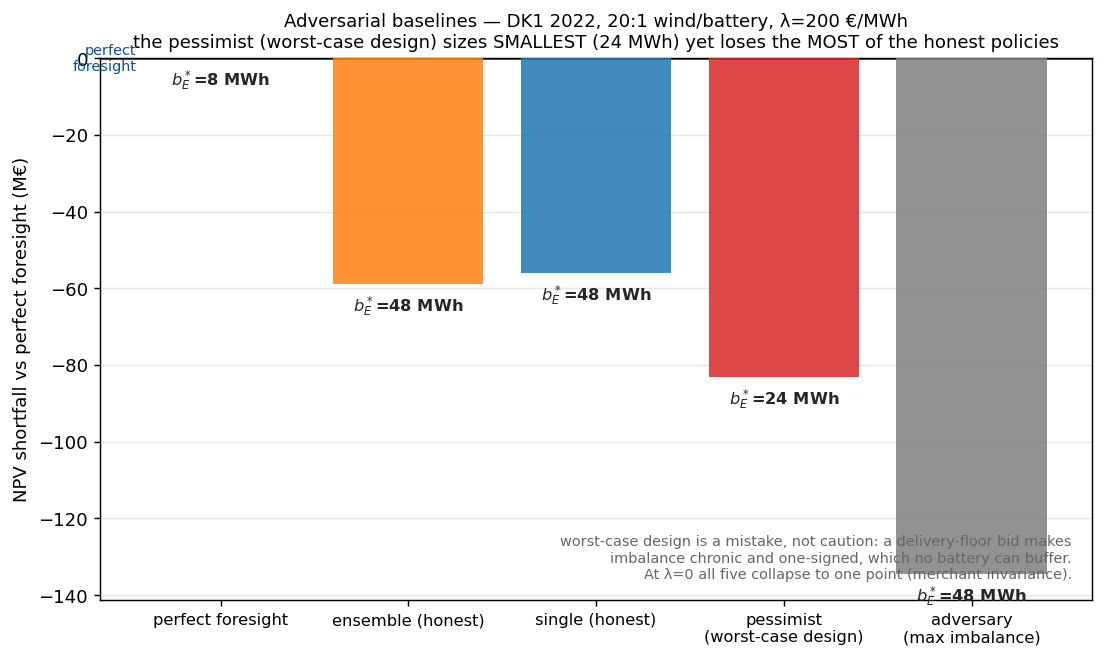
\includegraphics[width=0.8\textwidth]{fig_baselines.png}
\caption{\label{fig:baselines}Adversarial baselines in NPV-shortfall-below-perfect-foresight (DK1 2022, 20:1 wind/battery, $\lambda = 200$ EUR/MWh; the wind DA revenue $\sim 95$\,M\euro\ is differenced out so the battery economics are visible). Each bar is labelled with its optimal size. The pessimist (\texttt{adv\_design}, worst-case design) sizes \emph{smallest} ($24$ vs the honest $48$ MWh) yet loses the most of the honest policies --- a delivery-floor bid makes imbalance chronic and one-signed, which no battery can buffer, so worst-case design is a mistake rather than caution. At $\lambda = 0$ all five coincide (merchant invariance).}
\end{figure}

\begin{figure}[t]
\centering
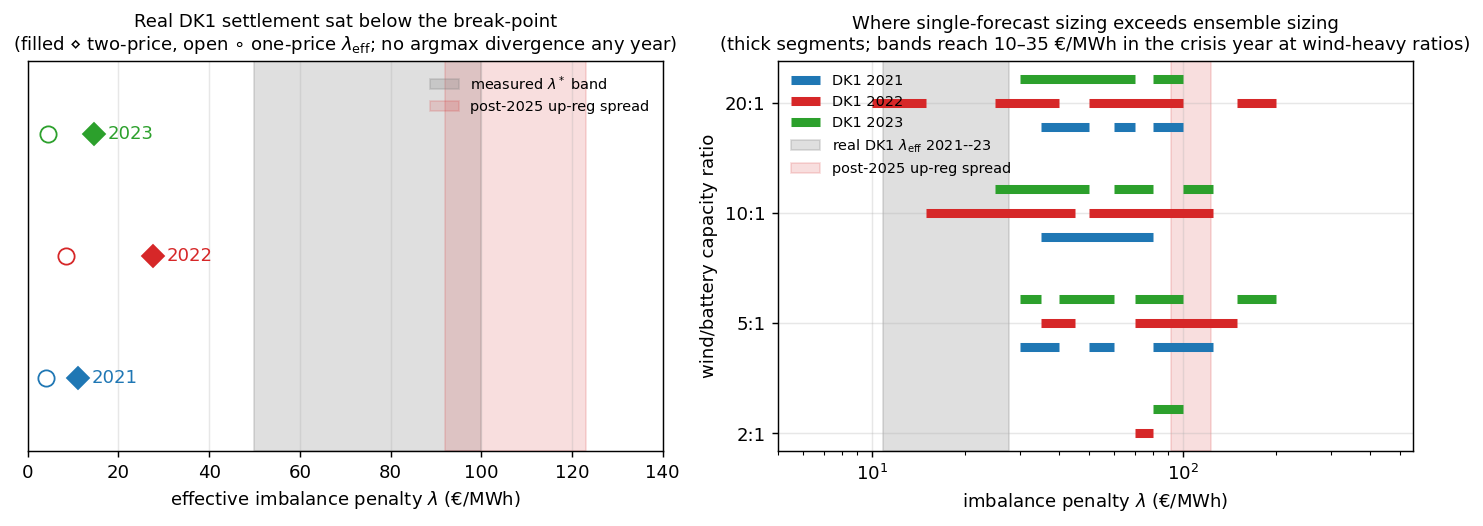
\includegraphics[width=0.95\textwidth]{fig_paper_real_imbalance.png}
\caption{\label{fig:realimbalance}Real-settlement anchor for the break-point study. Left: effective penalty $\lambda_{\mathrm{eff}}$ of actual DK1 imbalance settlement (eSett) per study year, against the measured break-point band and the post-March-2025 mean up-regulation spread; no argmax divergence occurs under real settlement in any year. Right: $\lambda$ ranges where the single-forecast policy sizes above the ensemble (thick segments, fine $\lambda$ grid, corrected settlement), by wind/battery ratio and year; bands open at $25$--$35$ EUR/MWh in normal years and reach $10$--$15$ in the 2022 crisis year at wind-heavy ratios. Real 2021--2023 settlement (grey) overlaps the crisis-year bands at wind-heavy ratios --- where real-settlement sizing indeed splits ($8$ vs $4$ MWh) --- and post-2025 spreads (red) sit deep inside the bands.}
\end{figure}

\subsection{Implication for sizing tools}

Across the markets and regimes tested, deterministic-LP-inner-dispatch in academic sizing tools (\texttt{hydesign}, \texttt{REopt}, \texttt{PyPSA}) is empirically robust on capacity recommendations \emph{at $\lambda = 0$}, and remained so under real DK1 settlement in normal years at every configuration tested; the 2022 crisis year split wind-heavy configurations only under a counterfactual two-price regime (retired November 2021), not under the in-force one-price regime. Operational stochastic dispatch is independently justified by the $0.9$--$37\%$ realized-NPV uplift at the recommended capacity. The $\lambda$-sweep of \S\ref{sec:imbalance} characterizes the regime where this conclusion is conditional: the imbalance cost gradient w.r.t.\ $b_E$ eventually dominates the deterministic-LP-vs-stochastic distinction, at $\lambda$ values that depend on wind sizing and forecast quality. The architectural divergence between commercial operational platforms and academic sizing tools is empirically supported on both DK1 and ERCOT --- not naive --- but its robustness is conditional on which side of $\lambda^*$ a given market sits.

This result cuts both ways for commercial positioning. Fluence markets Mosaic for \emph{pre-construction} use --- simulating assets ``to make better investment and operating decisions'' before breaking ground \citep{fluence2024mosaic}. In the merchant limit and in DK1 2021--2023, our data say stochastic dispatch fidelity changes the operating revenue but not the capacity recommendation; the pre-construction sizing value of stochastic simulation materializes only past $\lambda^*$. Conversely, the result refines a premise our own group put in print: \citet{assaad2025surrogate} motivated surrogate-based EMS modelling by the claim that low-fidelity inner operation ``leads to faulty sizing evaluations,'' while conceding the gap is hard to quantify. This paper supplies the quantification, and the answer is regime-dependent: the premise holds for operational NPV everywhere and for capacity above $\lambda^*$, but \emph{not} for capacity in the merchant limit --- where the cheap inner dispatch those surrogates replace was already sufficient for sizing. Related findings of fidelity-sensitive sizing in load-serving and system-scale settings \citep{dinh2025financial, cauz2023rl, schmidt2025foresight} are consistent with this regime structure: all sit on the penalized side of the boundary, where deviations from plan carry asymmetric cost.

\subsection{Limitations}

\begin{enumerate}
\item Sizing dimensionality in the imbalance extension. The 2-D $(b_E, b_P)$ stress test of \S\ref{sec:stress} covers the merchant limit only; the $\lambda > 0$ extension sweeps $b_E$ (and the wind ratio) at fixed $b_P = 1$ MW.
\item Multi-lag persistence is a weak ensemble. Modern probabilistic forecasts (deep quantile regression, ML weather) carry more information per member. The K=20 quantile-regression stress test addresses this at $\lambda = 0$ (and produced the single invariance break); the \emph{wind-side} forecasts in the imbalance extension remain persistence-only, so the $24$-vs-$16$ MWh gap is conditional on that choice. A skilled wind forecaster at $\lambda > 0$ is the most informative untested cell.
\item Scenario stochastic LP \citep{birge1997stochastic, krishnamurthy2018stochastic} was run only as a merchant-limit stress test (N=50, \S\ref{sec:stress}); production-grade SLP inside the imbalance extension is untested.
\item Replacement-count discreteness. Step changes can mask continuous shifts. Continuous-SoH model is future work.
\item No curtailment. The imbalance extension couples wind, but grid-cap-binding curtailment (a major HPP design driver) is absent; this paper isolates price-driven arbitrage plus imbalance absorption.
\item Two markets (DK1, ERCOT) at $\lambda = 0$; the real-settlement anchor is DK1-only, 2021--2023. Post-2025 DK1, Germany's reBAP, and Nord Pool 15-min settlement are the natural replications, and the diagnostic prescribes exactly that computation.
\item Dispatch is settlement-blind. The static-reserve settlement-aware class is tested (\S\ref{sec:imbalance}: headroom never pays below $\lambda = 500$, bands unchanged); dynamic bidding against imbalance-price forecasts is not, and could still shift the band.
\item Factorial dispatch is open-loop per chunk and therefore anticipative beyond 24 h (\S\ref{sec:setup}); revenue levels are upper bounds. The nonanticipative rolling SLP confirms the argmax but not the uplift magnitudes.
\end{enumerate}

The most consequential limitation is (2): a richer wind ensemble might move the break-point, in which case the diagnostic correctly fires under richer forecasts and the reported $\lambda^*$ is conditional on the cheap-ensemble baseline. We frame conservatively: \emph{multi-lag persistence ensemble does not break invariance on DK1 or ERCOT in the merchant limit, nor under real DK1 settlement 2021--2023, nor under a max-min robust decision rule over the same members, on the slices tested}.

\section{Conclusion}

We propose a regime-classification diagnostic for whether dispatch fidelity matters for battery sizing on a given market: the $b_{\mathrm{sat}}^\epsilon$ overlap test. The diagnostic is practitioner-runnable on one year of historical price data; it is falsifiable; and it survives independently of the theoretical proposition that motivates it. We test the diagnostic on synthetic, three years of DK1 (Energinet, including 2022 European energy crisis), and three years of ERCOT North Hub (gridstatus, including February 2021 Storm Uri). On every regime tested the diagnostic returns ``invariance survives'': $b_E^*$ is invariant across deterministic point-forecast, ensemble, scenario-stochastic, and max-min-robust dispatch, despite $0.9$--$37\%$ realized-NPV uplift at the optimum. The proposition predicted regime-dependent invariance breaking on multi-day spectral content; the data falsify the prediction. Coupling wind and imbalance settlement recovers the boundary of the invariance regime: persistent divergence bands opening at $25$--$35$ EUR/MWh in normal years and $10$--$15$ in the crisis year for wind-heavy plants. Settling against actual DK1 imbalance prices confirms both sides of the boundary: in normal years sizing is invariant at every configuration tested, while in the 2022 crisis year wind-heavy plants split ($8$ vs $4$ MWh) under a counterfactual two-price regime (retired November 2021) though not under the in-force one-price regime --- and the March-2025 Nordic balancing reforms sustain crisis-level spreads, making that divergence regime plausibly the post-reform normal. The architectural divergence between commercial operational platforms (Tesla / Fluence / W\"{a}rtsil\"{a}, all stochastic) and academic sizing tools (\texttt{hydesign} / \texttt{REopt} / \texttt{PyPSA}, all deterministic LP inner) is empirically supported across the regimes tested, with its boundary now mapped.

\paragraph{Reproducibility.}
Benchmark, four dispatch policies, multi-lag ensemble, sizing harness, pre-registration commits, and ERCOT + DK1 loaders are in \texttt{forecast-aware-sizing} at \url{https://github.com/kilojoules/forecast-aware-sizing} (commit hash in repo).

\appendix
\section{Supplementary figures}\label{app:supp}

The figures below provide the per-policy detail behind the stress-gauntlet
scoreboard (Figure~\ref{fig:gauntlet}) and the operational-lift summary
(Figure~\ref{fig:vss}). Each restates, at finer grain, an invariance the
scoreboard reports as a single cell; they are collected here to keep the
main-text figure arc focused on the adversarial ladder. Figure~\ref{fig:spectrum}
is the spectral motivation for the proposition the data falsify
(\S\ref{sec:falsify}).

\begin{figure}[h]
\centering
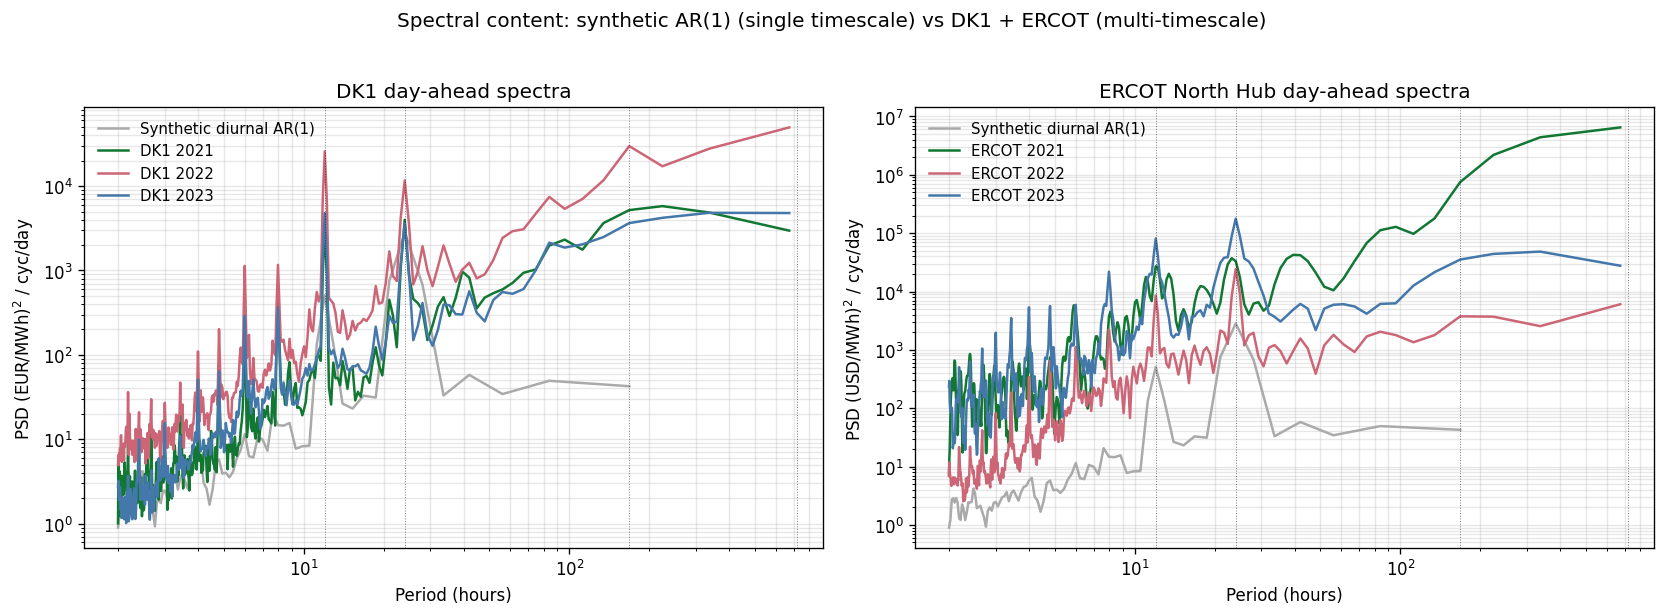
\includegraphics[width=0.8\textwidth]{fig_paper_spectrum.png}
\caption{\label{fig:spectrum}Welch PSD: synthetic vs DK1 + ERCOT day-ahead. Both real markets have substantial multi-day spectral weight; the proposition predicts invariance breaking, but \S\ref{sec:falsify} falsifies the prediction.}
\end{figure}

\begin{figure}[h]
\centering
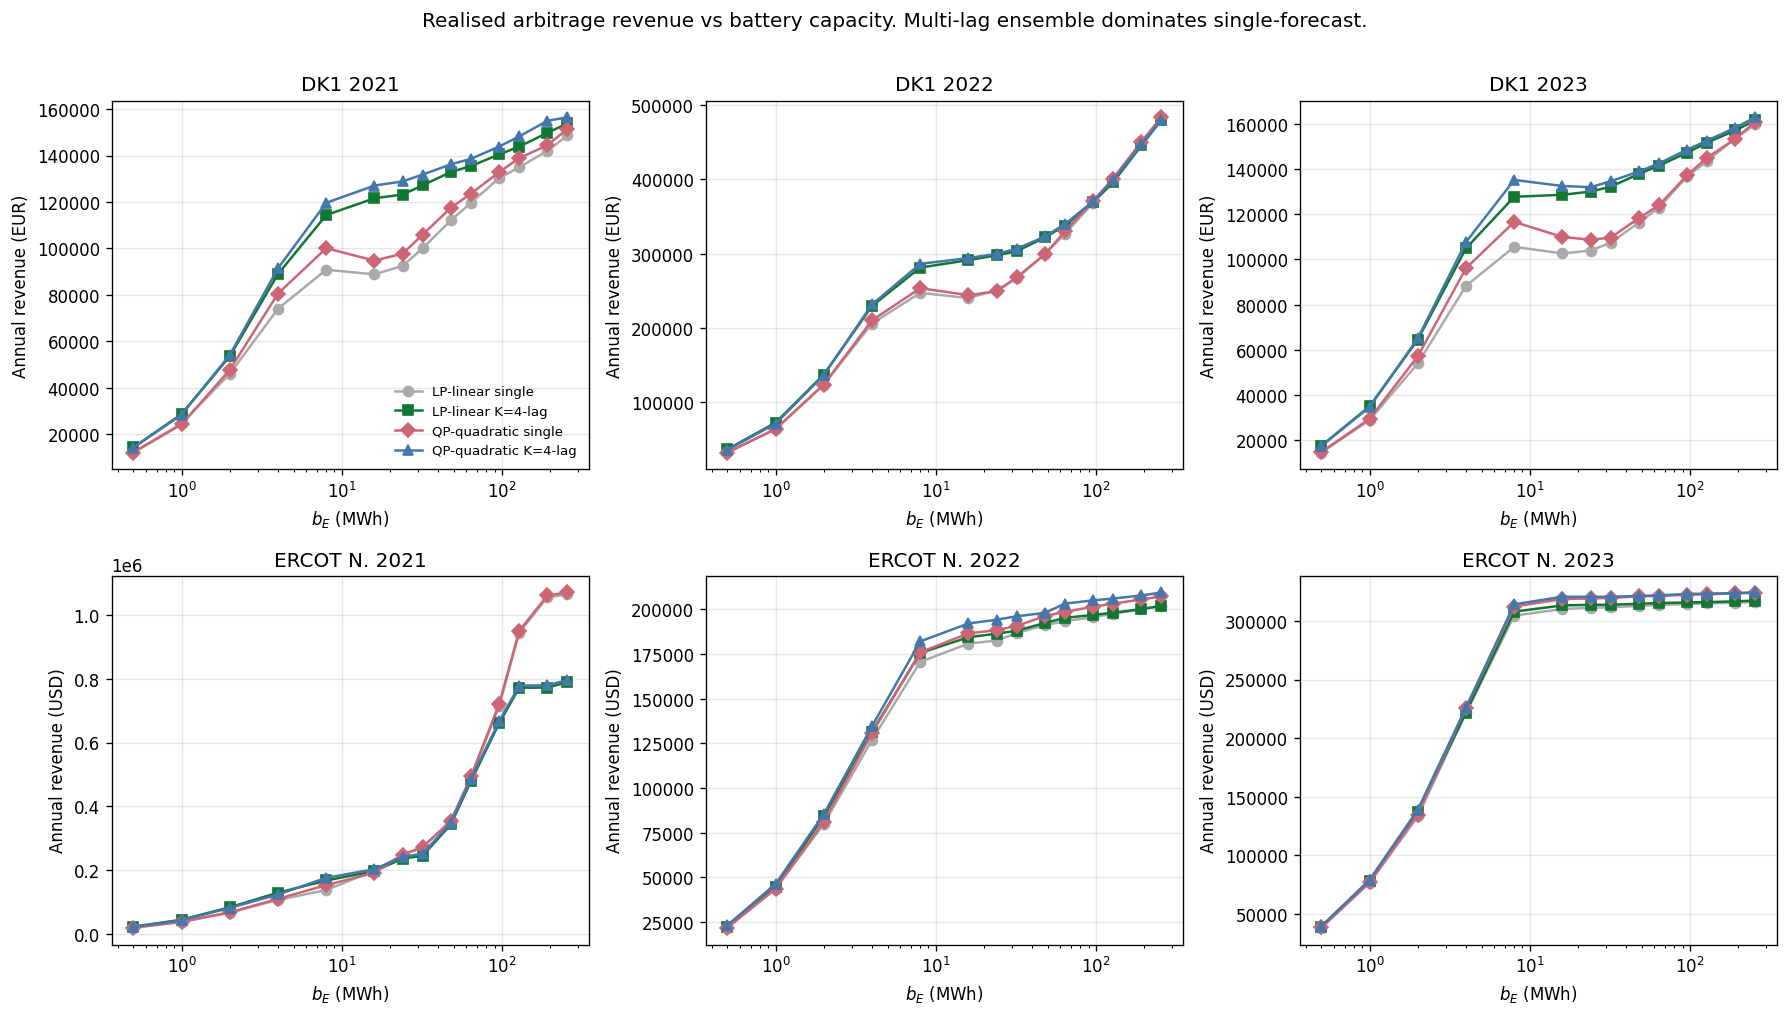
\includegraphics[width=0.9\textwidth]{fig_paper_revenue.png}
\caption{\label{fig:revenue}Annual realized revenue vs $b_E$. Multi-lag ensemble leads single-forecast in the relevant range. Past $b_E \sim 100$ MWh the curves cross --- ensemble's longer-period information is not net-positive at extreme capacity --- but this region is far past NPV-optimal.}
\end{figure}

\begin{figure}[h]
\centering
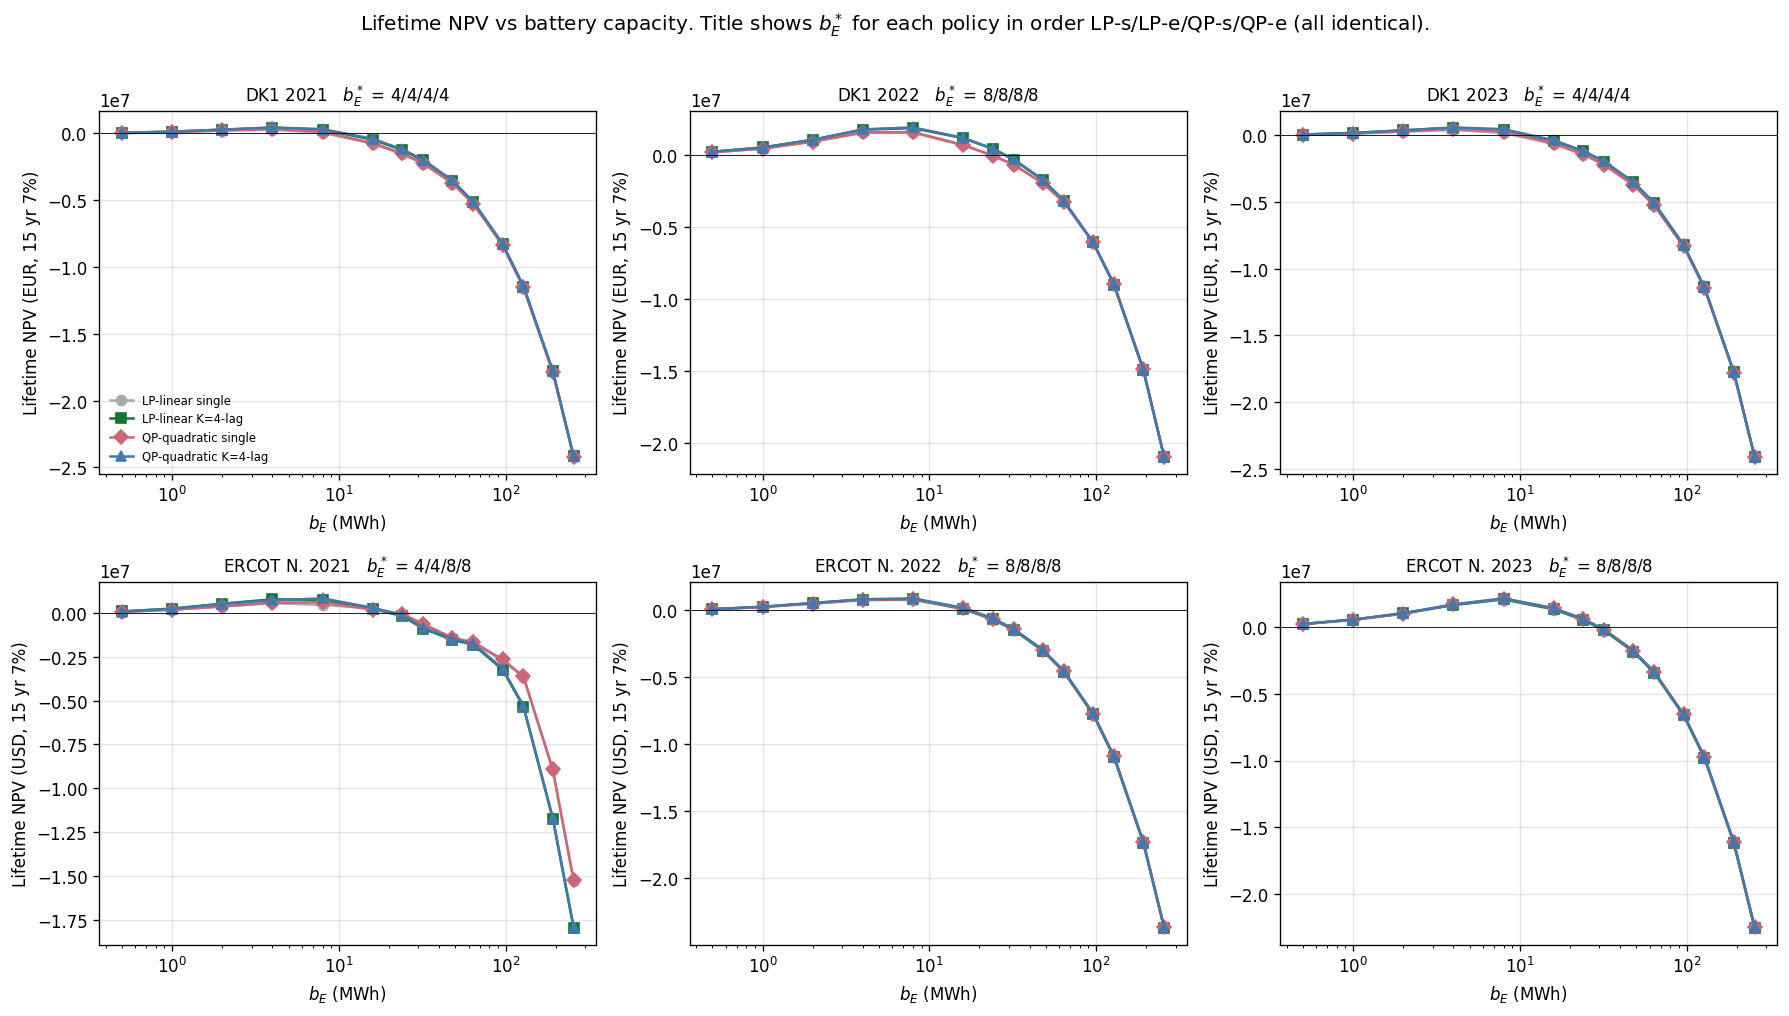
\includegraphics[width=0.9\textwidth]{fig_paper_npv.png}
\caption{\label{fig:npv}Lifetime NPV vs $b_E$ for DK1 by year. Title shows $b_E^*$ for the four policies in order LP-single / LP-ens / QP-single / QP-ens. All four are identical in every panel. ERCOT panels analogous. (Persistence-ensemble column of Figure~\ref{fig:gauntlet}.)}
\end{figure}

\begin{figure}[h]
\centering
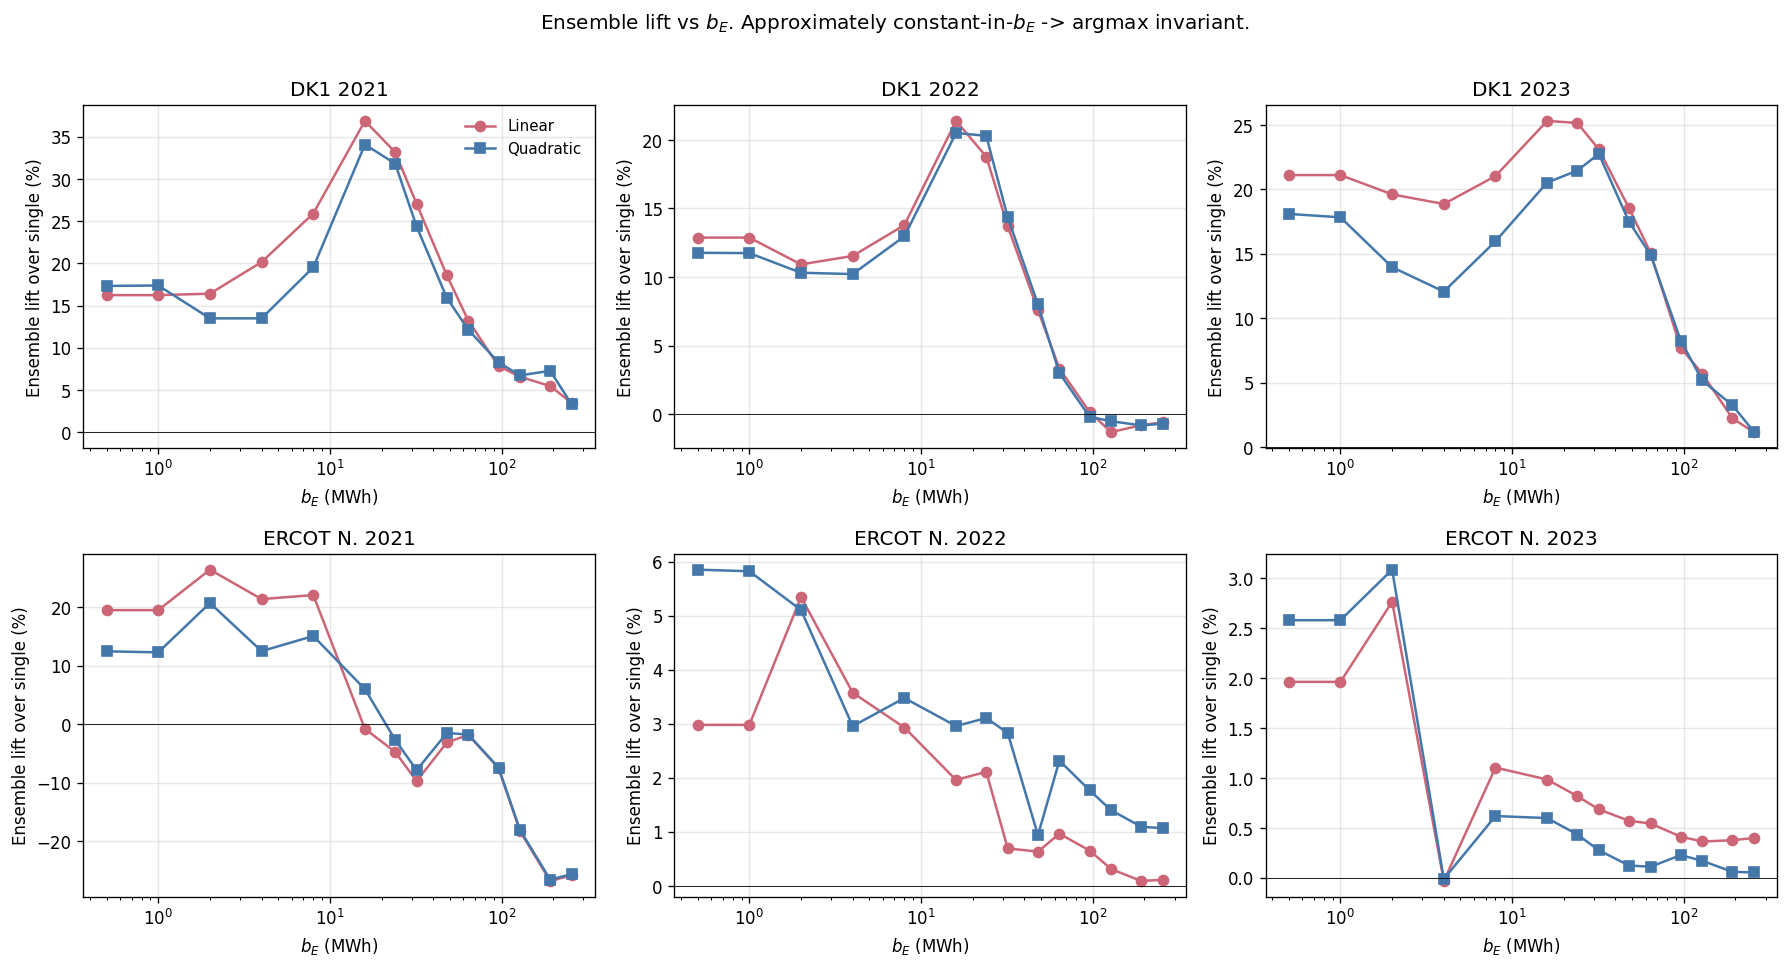
\includegraphics[width=0.9\textwidth]{fig_paper_lift.png}
\caption{\label{fig:lift}Ensemble revenue lift over single, by year (DK1). Approximately uniform in $b_E$ in the NPV-relevant range, supporting the empirical argmax-invariance.}
\end{figure}

\begin{figure}[h]
\centering
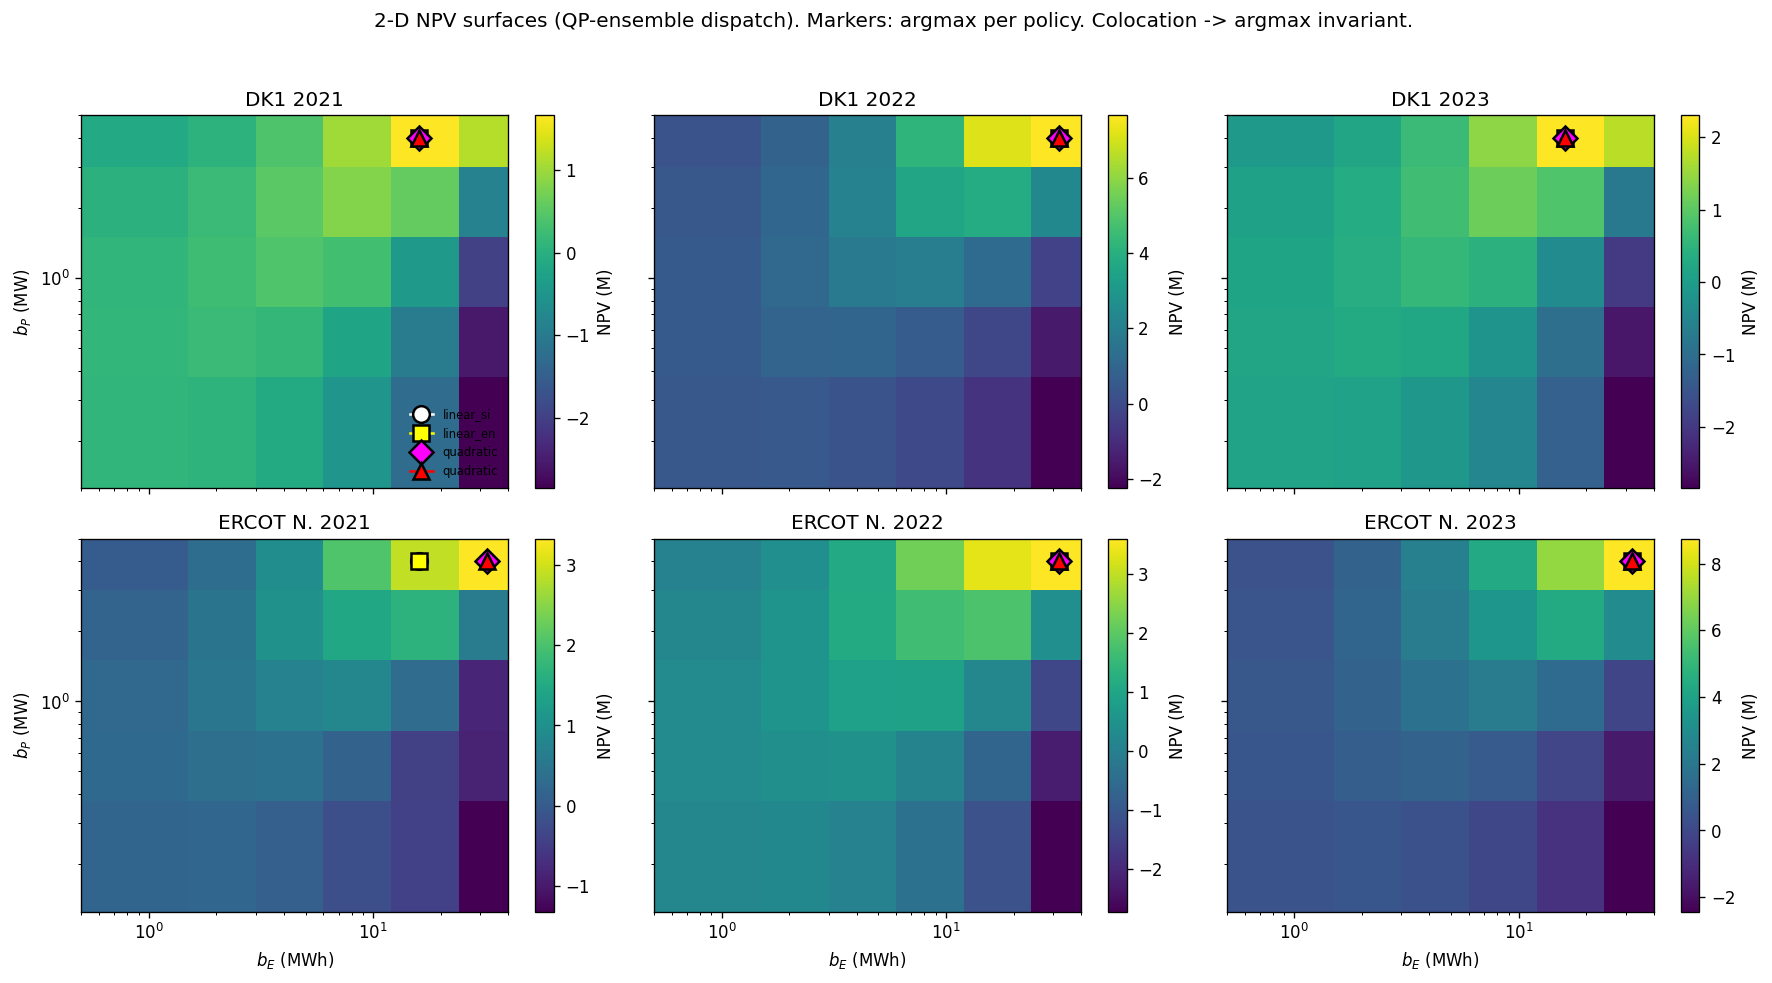
\includegraphics[width=0.9\textwidth]{fig_paper_2d.png}
\caption{\label{fig:2d}2-D NPV surfaces (QP-ensemble dispatch). Markers show argmax for each of the 4 policies; they coincide at the same $(b_P^*, b_E^*)$ cell in every (market, year) panel (2-D column of Figure~\ref{fig:gauntlet}). Most argmaxes land at the corner of the tested grid, suggesting the actual optimum lies past our range.}
\end{figure}

\begin{figure}[h]
\centering

\includegraphics[width=0.9\textwidth]{fig_paper_slp.png}
\caption{\label{fig:slp}Two-stage rolling-horizon stochastic LP (N=50 scenarios per 24-h window, green) vs full-horizon QP-single and QP-ensemble. SLP NPV is lower (rolling vs perfect-foresight gap); argmax $b_E^*$ matches the linear policies in every market-year, sitting one grid step below the full-horizon QP argmax at ERCOT 2021 (the \ding{55} on the gauntlet's SLP column).}
\end{figure}

\begin{figure}[h]
\centering
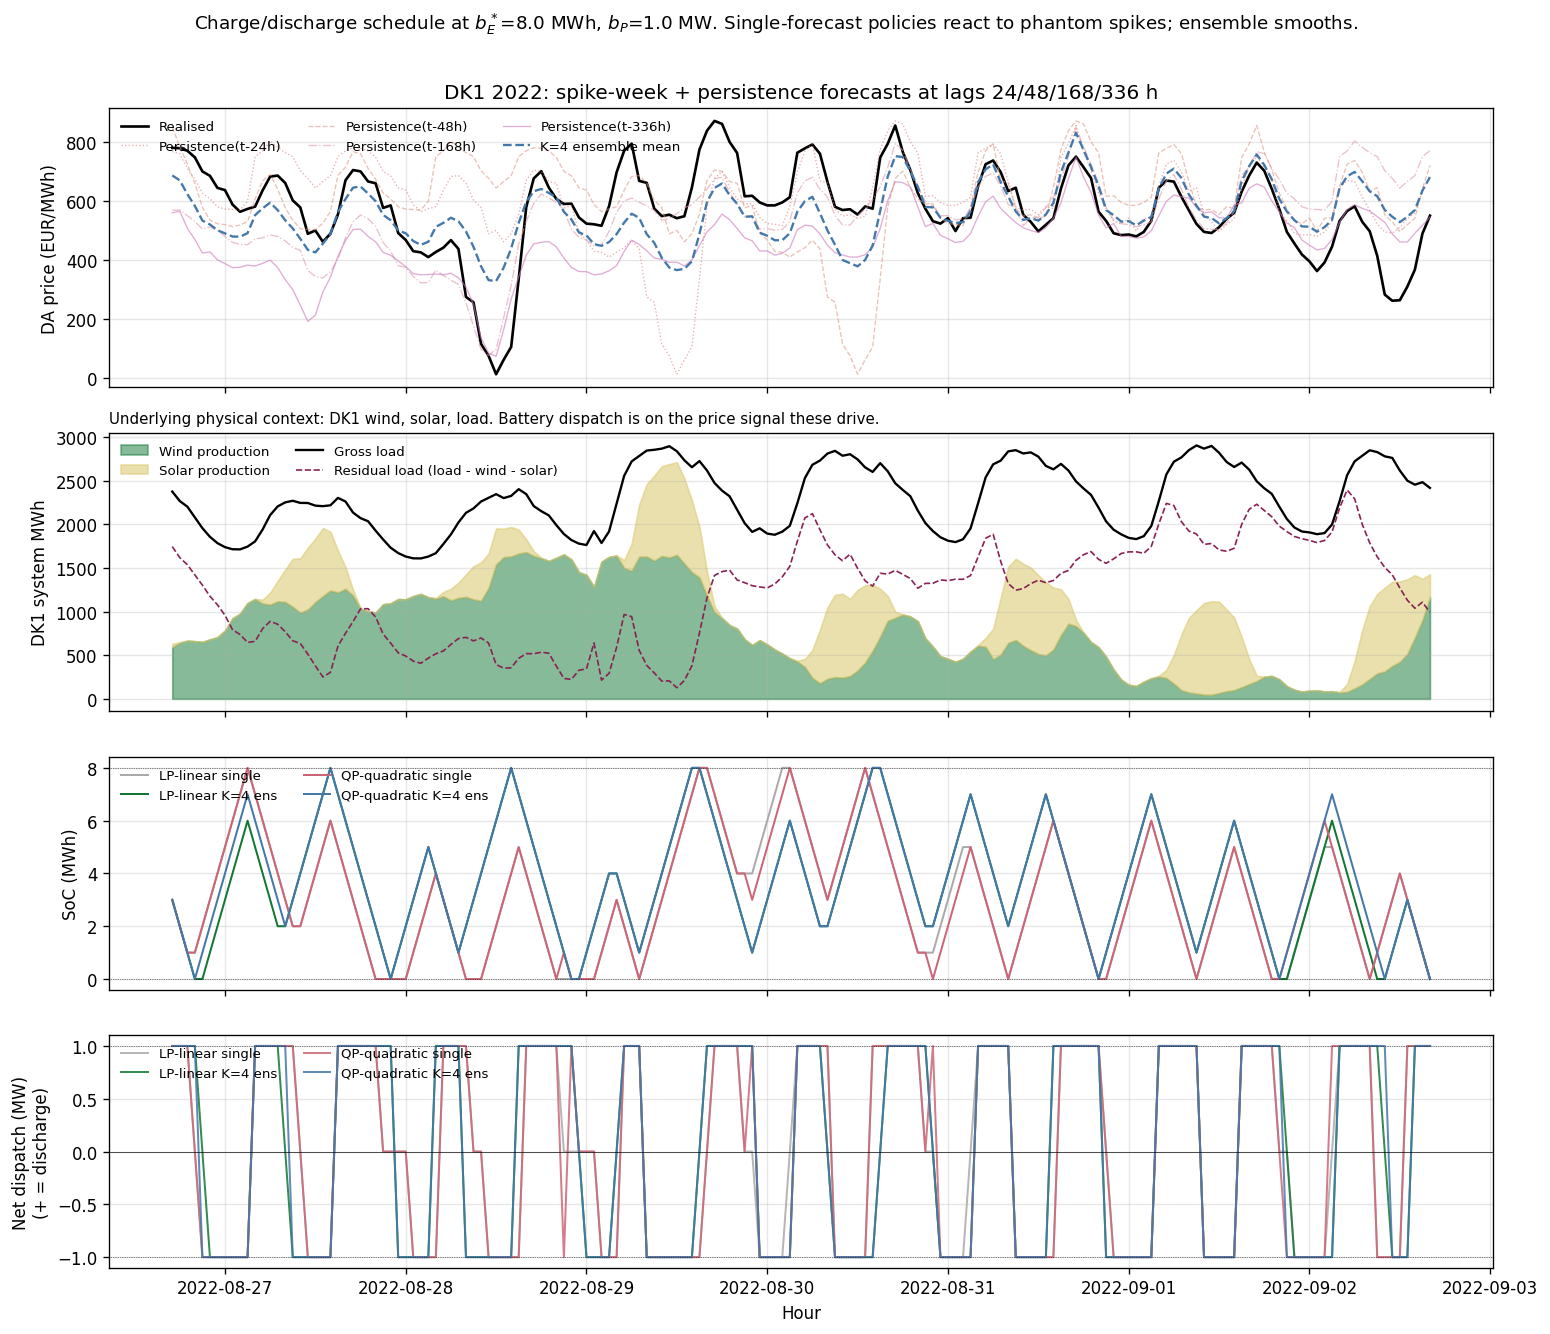
\includegraphics[width=0.9\textwidth]{fig_paper_timeseries.png}
\caption{\label{fig:timeseries}DK1 2022 spike week (max price \euro 871/MWh, 2022-09-01). Top: realized DA price + multi-lag persistence forecasts + ensemble mean. Second: physical context. Third: SoC under each of 4 policies (overlapping). Bottom: net dispatch (overlapping). The policies make near-identical decisions, the merchant-limit similarity the diagnostic measures.}
\end{figure}

\bibliographystyle{plainnat}
\begin{thebibliography}{99}

\bibitem[Assaad et al., 2025]{assaad2025surrogate}
Assaad, C., Murcia Le\'{o}n, J.\,P., Quick, J., G\"{o}\c{c}men, T., Ghazouani, R., Das, K.\ (2025). Enabling efficient sizing of hybrid power plants: a surrogate-based approach to energy management system modeling. \emph{Wind Energy Science}, 10:559--578.

\bibitem[Birge \& Louveaux, 1997]{birge1997stochastic}
Birge, J.\,R., Louveaux, F.\ (1997). \emph{Introduction to Stochastic Programming}. Springer.

\bibitem[Bludszuweit \& Dom\'{i}nguez-Navarro, 2011]{bludszuweit2011probabilistic}
Bludszuweit, H., Dom\'{i}nguez-Navarro, J.\,A.\ (2011). A probabilistic method for energy storage sizing based on wind power forecast uncertainty. \emph{IEEE Transactions on Power Systems}, 26(3):1651--1658.

\bibitem[Blue Power Partners, 2025]{bluepower2025}
Blue Power Partners (2025). Danish imbalance costs surge following market design changes. \url{https://bluepowerpartners.com/danish-imbalance-costs-surge-following-market-design-changes/}.

\bibitem[Cauz et al., 2023]{cauz2023rl}
Cauz, M., Bolland, A., Miftari, B., Perret, L., Ballif, C., Wyrsch, N.\ (2023). Reinforcement learning for joint design and control of battery-PV systems. \emph{Proc.\ ECOS 2023}; arXiv:2307.04244.

\bibitem[Cao et al., 2020]{cao2020drl}
Cao, J., Harrold, D., Fan, Z., Morstyn, T., Healey, D., Li, K. (2020). Deep Reinforcement Learning-Based Energy Storage Arbitrage With Accurate Lithium-Ion Battery Degradation Model. \emph{IEEE Transactions on Smart Grid}, 11(5):4513--4521.

\bibitem[Dinh et al., 2025]{dinh2025financial}
Dinh, H.\,T., Karimi-Arpanahi, S., Pourmousavi, S.\,A., Guo, R., Lemos-Vinasco, J., Liisberg, J.\,A.\ (2025). On the financial consequences of simplified battery sizing models without considering operational details. \emph{Journal of Energy Storage}; arXiv:2310.02494.

\bibitem[Energinet, 2024]{energinet2024}
Energinet (2024). Elspotprices public dataset. \url{https://www.energidataservice.dk/tso-electricity/elspotprices}.

\bibitem[eSett, 2026]{esett2026}
eSett Oy (2026). Nordic imbalance settlement open data: imbalance and regulation prices. \url{https://opendata.esett.com/}.

\bibitem[Fluence, 2024]{fluence2024mosaic}
Fluence Energy (2024). Mosaic Intelligent Bidding Software. \url{https://fluenceenergy.com/mosaic-intelligent-bidding-software/}.

\bibitem[gridstatus.io, 2024]{gridstatus2024}
gridstatus.io (2024). Open-source Python wrapper for ISO market data. \url{https://github.com/gridstatus/gridstatus}.

\bibitem[Haessig et al., 2015]{haessig2015storage}
Haessig, P., Multon, B., Ben Ahmed, H., Lascaud, S., Bondon, P.\ (2015). Energy storage sizing for wind power: impact of the autocorrelation of day-ahead forecast errors. \emph{Wind Energy}, 18(1):43--57.

\bibitem[Hong et al., 2014]{hong2014global}
Hong, T., Pinson, P., Fan, S. (2014). Global energy forecasting competition 2012. \emph{International Journal of Forecasting}, 30(2):357--363.

\bibitem[Krishnamurthy et al., 2018]{krishnamurthy2018stochastic}
Krishnamurthy, D., Uckun, C., Zhou, Z., Thimmapuram, P., Botterud, A.\ (2018). Energy storage arbitrage under day-ahead and real-time price uncertainty. \emph{IEEE Transactions on Power Systems}, 33(1):84--93.

\bibitem[Mokhtare et al., 2024]{mokhtare2024offshore}
Mokhtare, Z., et al.\ (2024). Optimal sizing of battery energy storage system for a large-scale offshore wind power plant considering wind uncertainty and penalty factors. \emph{IET Renewable Power Generation}. doi:10.1049/rpg2.12970.

\bibitem[Murcia Le\'{o}n et al., 2024]{murcia2024hydesign}
Murcia Le\'{o}n, J.\,P., Habbou, H., Friis-M\o ller, M., Gupta, M., Zhu, R., Das, K.\ (2024). HyDesign: a tool for sizing optimization of grid-connected hybrid power plants. \emph{Wind Energy Science}, 9:759--776.

\bibitem[NREL, 2025]{nrel2025bessdeg}
National Renewable Energy Laboratory (2025). Battery Degradation Modeling in Hybrid Power Plants. NREL/TP-FY25-84791.

\bibitem[Pinson et al., 2007]{pinson2007trading}
Pinson, P., Chevallier, C., Kariniotakis, G.\,N.\ (2007). Trading wind generation from short-term probabilistic forecasts of wind power. \emph{IEEE Transactions on Power Systems}, 22(3):1148--1156.

\bibitem[Schmidt, 2025]{schmidt2025foresight}
Schmidt, F.\ (2025). On long-duration storage, weather uncertainty and limited foresight. arXiv:2505.12538.

\bibitem[Shi et al., 2017]{shi2017convex}
Shi, Y., Xu, B., Wang, D., Zhang, B.\ (2017). Using Battery Storage for Peak Shaving and Frequency Regulation: Joint Optimization for Superlinear Gains. \emph{arXiv:1703.07968}.

\bibitem[Tesla, 2024]{tesla2024autobidder}
Tesla, Inc.\ (2024). Autobidder Support Documentation. \url{https://www.tesla.com/support/energy/tesla-software/autobidder}.

\bibitem[W\"{a}rtsil\"{a}, 2025]{wartsila2025gems}
W\"{a}rtsil\"{a} Energy (2025). GEMS Pulse press release.

\bibitem[Weron, 2014]{weron2014electricity}
Weron, R.\ (2014). Electricity price forecasting: a review of the state-of-the-art. \emph{International Journal of Forecasting}, 30(4):1030--1081.

\bibitem[Xu, 2018]{xu2018modeling}
Xu, B.\ (2018). \emph{Modeling and Control of Energy Storage Systems for Power System Operations}. PhD thesis, University of Washington.

\end{thebibliography}

\end{document}
